\documentclass[14pt, dvipsnames]{extarticle}
\usepackage[left=2cm, top=2cm, right=2cm, bottom=20mm]{geometry} 
\usepackage[utf8x]{inputenc} % Включаем поддержку UTF8
\usepackage[russian]{babel}  % Включаем пакет для поддержки русского языка
\usepackage{ucs}
\usepackage{tikzsymbols}
 \usepackage{fontawesome}
 \usepackage{simpsons}
 \usepackage{xcolor}
  \usepackage{stackrel}
 
\usepackage{wrapfig}
  
\usepackage{amsthm, amsmath, amssymb} % Mathematical typesetting
\usepackage{hyperref} % For hyperlinks in the PDF

\usepackage{esint}
 
\newtheorem{theorem}{Теорема}
\newtheorem{statement}{Утверждение}
\newtheorem{proposition}{Предложение}
\newtheorem{lemma}{Лемма}
\newtheorem{corollary}{Следствие}[theorem]
\newtheorem{question}{\sc Вопрос}


\theoremstyle{definition}
\newtheorem{defi}{Определение}
\newtheorem{property}{Свойство}
\newtheorem{problem}{Задача}
\newtheorem{exercise}{Упражнение}
\newtheorem{example}{Пример}

\theoremstyle{remark}
\newtheorem*{comment}{Замечание}

\usepackage{enumerate}




\usepackage{fancybox,fancyhdr}
\usepackage{lipsum}
\fancyhead[R]{}
\fancyhead[C]{\sc\leftmark}
\fancyhead[L]{}
%\renewcommand{\headrulewidth}{0.5pt}
%\renewcommand{\footrulewidth}{0.5pt}
\fancyfoot[C]{\hrulefill\protect\circled{\thepage}\hrulefill}

\usepackage{tikz}
\newcommand*\circled[1]{\tikz[baseline]{\node[shape=circle,draw,inner sep=2pt] (char) {#1};}}






\usepackage{asymptote}

\usepackage[all]{xy}

\DeclareMathOperator{\Tor}{\mathrm{Tor}\!}
\DeclareMathOperator{\End}{\mathrm{End}\,}
\DeclareMathOperator{\Sq}{\mathrm{Sq}}
\DeclareMathOperator{\cp}{\smallsmile}
\DeclareMathOperator{\Hom}{\mathrm{Hom}}
\DeclareMathOperator{\Sp}{\mathrm{Sp}}
\DeclareMathOperator{\Z2}{\mathbb{Z}_2}
\DeclareMathOperator{\Ho}{\mathrm{Ho}}
\DeclareMathOperator{\CC}{\mathbb{C}\!}
\DeclareMathOperator{\Hig}{\mathrm{Hig}}

\renewcommand{\phi}{\varphi}

\usepackage{textcomp}

\usepackage{mathabx}

%Некий костыль с двух сторон от декларации пакета bm
\let\saveboldsymbol\boldsymbol
\usepackage{bm}
\let\boldsymbol\saveboldsymbol

\usepackage{mathrsfs} 

\usepackage{indentfirst}

\newcommand{\factor}[2]{{\raisebox{.2em}{$#1$}\left/\raisebox{-.2em}{$#2$}\right.}}

\usepackage{titlesec}
\titleformat{\section}
  {\normalfont\Large\bfseries}{\S\thesection}{1em}{}
  
  
  \title{Топологические инварианты конечно определённых групп}
  
  \date{}


\begin{document}

\maketitle

\section{Введение}

Д. Кан и У. Тёрстон доказали (\cite{Kan}, 1976), что (ко)гомологии классифицирующего пространства $K(G, 1)=:TX$ дискретной группы $G$ могут быть такими, как у произвольного линейно связного пространства $X$. Причём отображение $t: TX \to X$ естественно по $X$, и $T$ является функтором.

В той же работе было отмечено, что функтор $T$ и функтор плюс-конструкции Квиллена $(\cdot)^+$ в некотором смысле взаимно обратны. Они устанавливают эквивалентность категории гомотопий CW-комплексов и локализации категории $GP$. Объектами последней являются пары $(G, P)$, где $P$ — совершенная нормальная подгруппа группы $G$, а морфизмами являются такие гомомофризмы $f: (G, P) \to (G’, P’)$, что $f(P) < P’$. Локализация происходит по тем морфизмам категории $GP$, которые индуцируют изоморфизмы на фактор группах $G/P \to G’/P’$ и на гомологиях $H(G; A) \to H(G’; A)$. Таким образом, теория гомотопий CW-комплексов восстанавливается из теории дискретных групп.   

Классифицирующие пространства групп имеют большое значение в топологии и алгебре. Известное множество их конструкций: например, конструкция Милнора \cite{MilnorBar}, конструкция Милграма \cite{Milgram}, категорный подход через симплициальные множества \cite{Lenz} и др. Интересно было бы найти обозримую симплициальную функториальную конструкцию классифицирующих пространств групп. Это бы позволило, например, подойти к определению торических (ко)гомологий конечно определённых групп: их можно было бы определить, как (ко)гомологии момент-угол комплекса, построенного по симплициальному классифицирующему пространству данной группы. 

Важно заметить также, что имеются модификации конструкция Кана --- Тёрстона, которые для конечных CW-комплексов дают дискретные группы, классифицирующие пространства которых являются конечными клеточными комплексами \cite{BDH}, \cite{Maunder}. Проблема геометрической размерности дискретных групп имеет давнюю историю. Известная теорема Эйленберга --- Ганея \cite{Ganea} утверждает, что для любой конечно определённой группы $G$ когомологической размерности не больше $n$, где $n ≥ 3$, существует асферичный $n$-мерный CW-комплекс $X = K(G, 1)$. Для $n = 2$ — это гипотеза, открытая и по настоящее время.

С конструкцией Кана-Тёрстона тесно связаны ацикличные дискретные группы. Они могут возникать, как фундаментальные группы $n$-узлов, гомологических сфер, как группы гомеоморфизмов многообразий, возникают в теории слоений \cite{Berrick} и др. Большой интерес представляют конечно определённые ацикличные группы. Одним из простейших нетривиальных примеров \cite{Higman} являются группы Хигмана $\mathrm{Hig}_n$, $n=4, 5, ...$,. Эти группы замечательны ещё и тем, что они имеют конечную геометрическую размерность: их классифицирующим пространством может быть выбран конечный двумерный клеточный комплекс \cite{BDH}. Ацикличные пространства и группы дают надежду на обобщение классических конструкций топологии. Например, можно попробовать обобщить конструкции, в которых участвуют стягиваемые пространства, заменив последние некоторым образом на ацикличные пространства.

Можно задаться вопросом о том, когда данная ацикличная группа имеет конечную геометрическую размерность. Дополнительную сложность задаче придаёт то, что когомологическая размерность равна 0. Однако, как показали Уолл и Милнор, препятствием пространству $X$ быть гомотопически эквивалентным конечному комплексу служит так называемое кручение Уайтхеда $\mathrm{Wh}_0(\mathbb{Z}[\pi_1(X)])$ группового кольца $\mathbb{Z}[\pi_1(X)]$. 

Близким к данному кругу вопросов являются вопросы о классифицирующих пространствах моноидов. В этом контексте можно упомянуть гипотезу Арнольда-Тома-Фама \cite{Dobr} и проблему Бёрнсайда \cite{Burnside}. 



\section{Напоминание о гомологиях дискретных групп}

По данной дискретной группе $G$ можно, как известно, построить стягиваемый симплициальный комплекс $EG$ со свободным действием $G$. Факторпространство $BG:=\factor{EG}{G}$ называется {\it классифицирующим пространством} группы $G$. 

Классифицирующее пространство дискретной группы $G$ имеет тип $K(G, 1)$.

\begin{defi}
Гомологиями дискретной группы $G$ с тривиальными коэффициентами в $\mathbb{Z}$ называются гомологии (симплициальные, клеточные и др.) классифицирующего пространства группы $G$, то есть $H_i(G; \mathbb{Z}):=H_i(BG; \mathbb{Z})$. В случае локальных коэффициентов в $G$-модуле $M$ это гомологии с локальными коэффициентами $H_i(BG; M)$.
\end{defi}



Существуют различные конструкции классифицирующих пространств для топологических и дискретных групп. Сюда относится конструкция с джойнами Милнора, бар-конструкция, конструкция Милграма, категорная конструкция через геометрическую реализацию некоторого симплициального множества и др.

Также гомологии группы $G$ могут быть определены чисто алгебраическим путём.

\begin{defi}
Гомологиями дискретной группы с коэффициентами в $G$-модуле $M$ называются группы $H_n(G, M)=\mathrm{Tor}^{\mathbb{Z}[G]}_n(\mathbb{Z}, M)$.
\end{defi}


\begin{statement}
Два определения гомологий групп равносильны.
\end{statement}

%С каждым гомоморфизмом групп $G_1\to G_2$ связано расслоение $\factor{G_2}{G_1}\to BG_1\to BG_2$.






\section{Ацикличные группы}

 Имеется интересный класс групп, гомологии которых в $\mathbb{Z}$ устроены, как гомологии точки. Такие группы называются {\it ацикличными}. 
 
 Заметим, что ацикличных групп в любой локальной системе коэффициентов не существует, поскольку имеет место
 
 \begin{theorem}[Столлингс ???]
 Если когомологическая размерность конечно порождённой группы $G$ не превосходит 1, то $G$ является свободной (т. е. $K(G, 1)$ гомотопически эквивалентно букету окружностей).
 \end{theorem}
 


\subsection{Примеры ацикличных дискретных групп}

В этом параграфе приводятся два примера конечно представленных ацикличных групп, классифицирующие пространства которых могут быть реализованы двумерными симплициальными комплексами. 

\paragraph{Группа $\mathfrak{A}$.} 


Рассмотрим простой пример нетривиальной ацикличной группы --- группу $\mathfrak{A}$ из статьи \cite{BDH}.

Для её построения сначала введём две группы: $$F=\langle a, b \rangle,$$ $$C=\langle u=a,\ v=b^{-1}a^{-1}bab,\ w=b^{-2}ab^{-1}a^{-2}bab^2,\ x= b^{-3}ab^{-1}a^{-2}bab^3 \rangle.$$

Группа $F$ --- свободная на двух образующих, а группа $C$ --- свободная на четырёх образующих.

При помощи $F$ и $C$ мы можем получить группу $$\mathfrak{A}=\{ F_1\star F_2; C_1\cong_\varphi C_2\},$$ где $F_1, \ F_2$ --- две копии группы $F$, а $C_1$, $C_2$ --- копии группы $C$, причём склейка происходит вдоль изоморфизма $\varphi: C_1\to C_2$, такого, что $$u_1\mapsto x_2,\ v_1\mapsto w_2,\ w_1\mapsto v_2,\ x_1\mapsto u_2.$$ 

\begin{statement}
Группа $\mathfrak{A}$ нетривиальна.
\end{statement} 

\begin{proof}
Как известно, свободные группы нетривиальны. Но результат амальгамированного произведения двух нетривиальных групп по их общей подгруппе будет нетривиальной группой. Последнее следует, например, из теории Басса-Серра (см., например, [???]).
\end{proof}

\begin{statement}[\cite{BDH}] 
Группа $\mathfrak{A}$ является ацикличной.
\end{statement}

\begin{proof}

По построению группа $\mathfrak{A}$ является совершенной.

Кроме того, пространство $K(\mathfrak{A}, 1)$ можно реализовать в виде конечного клеточного двумерного комплекса, поскольку он является пушаутом двух копий  пространства $K(F, 1)\simeq \mathbb{S}^1\vee \mathbb{S}^1$ вдоль пространства $K(C, 1)\simeq \mathbb{S}^1\vee\mathbb{S}^1\vee\mathbb{S}^1\vee\mathbb{S}^1$, то есть $$K(\mathfrak{A}, 1)=K(F, 1)\sqcup_{K(C, 1)} K(F, 1).$$ 

Имеет место точная последовательность Майера-Виеториса с постоянными коэффициентами в $\mathbb{Z}$ 
$$...\to H_{n+1}\mathfrak{A}\to H_nC\to H_nF_1\oplus H_n F_2\to H_n\mathfrak{A}\to ...$$

В силу того, что $K(F, 1)$ и $K(C, 1)$ --- букеты окружностей, сразу получается, что $H_n\mathfrak{A}=0$ при $n>2$. Рассмотрим теперь участок точной последовательности для случая $n=2$: 
$$0\to H_2\mathfrak{A}\to H_1C\to H_1F_1\oplus H_1F_2\to 0.$$ Но обе свободные абелевы группы $H_1C$ и $H_1F_1\oplus H_1 F_2$ имеют ранг 4. Следовательно, они изоморфны, и $H_2\mathfrak{A}=0$ в силу точности.


\end{proof}

Для дальнейшего нам понадобится важная

\begin{theorem}[Дж. Уайтхед, 1939]\label{Whitehead}
Пусть группа $G$ является pushout'ом в категории $\mathsf{Grp}$ в следующей диаграмме 

$$\xymatrix{
    C \ar@{^{(}->}[r] \ar@{^{(}->}[d] & A \ar[d] \\
    B \ar[r]       & G }$$ 
    
Тогда следующая диаграмма является pushout'ом в категории $\mathsf{Top}$ 

$$\xymatrix{
    K(C, 1) \ar[r] \ar[d] & K(A, 1) \ar[d] \\
    K(B, 1) \ar[r]       & K(G, 1) }$$ 
    
\end{theorem}

\begin{corollary}[\cite{BDH}]\label{finite}
Если $G=A\star_C B$ является амальгамой групп $A$ и $B$, для которых существуют конечные симплициальные реализации пространств $K(A, 1)$, $K(B, 1)$ и $K(C, 1)$, тогда $K(G, 1)$ тоже может быть реализовано в виде конечного симплициального комплекса. Причём имеет место оценка на размерности $$\dim G\leqslant \max(\dim A, \dim B, 1+\dim C).$$
\end{corollary} 

\begin{proof}

Вложениям $C\hookrightarrow A$ и $C\hookrightarrow B$ соответствуют отображения классифицирующих пространств $K(C, 1)\to K(A, 1)$ и $K(C, 1)\to K(B, 1)$. Возьмём цилиндры этих отображений и склеим их вдоль комплекса $K(C, 1)$.
\end{proof}

Отсюда получается  

\begin{statement}
Группа $\mathfrak{A}$ является ацикличной относительно тривиальной системы коэффициентов в $\mathbb{Z}$ и может быть реализована в виде конечного двумерного клеточного комплекса.
\end{statement}











\paragraph{Группы Хигмана $\mathrm{Hig}_n$.}

Эти группы были придуманы Г. Хигманом в работе \cite{Higman}, 1951, как примеры конечно определённых групп, не имеющих подгрупп конечного индекса.

Рассмотрим сначала группу

$$\mathrm{Hig}_4=\langle a, b, c, d\ |\ a^{-1}ba=b^2, b^{-1}cb=c^2, c^{-1}dc=d^2, d^{-1}ad=a^2 \rangle.$$ 

Опишем, как можно получить эту группу при помощи операций HNN-расширения и амальгамированного свободного произведения.

Рассмотрим группу Баумслага-Солитера: $$\mathrm{BS}(1,2)=K=\langle a, b | a^{-1}ba=b^2 \rangle.$$

Можно заметить, что группа $K$ является HNN-расширением группы $\langle b \rangle\cong\mathbb{Z}$ при помощи изоморфизма подгрупп $\langle b \rangle \cong \langle b^2 \rangle$. В первую очередь, группа $K$ ненулевая по лемме Бриттона, поскольку в неё вкладывается группа $\langle a \rangle$. 

%Также из леммы Бриттона следует, что если бы $K$ имела элемент кручения, то он был бы сопряжён некоторому элементу группы $\mathbb{Z}$, значит, $K$ не имеет кручения.  

Дайер и Васкез показали, что верна

\begin{theorem}[E. Dyer, A. T. Vasquez, 1972, \cite{Vasquez}]

Пусть $P=\langle A\ |\ R \rangle$ --- представление группы $G$ с одним соотношением. Тогда клеточный 2-комплекс, получаемый обычной приклейкой 2-клетки к букету окружностей, биективно соответствующих образующим из $A$ вдоль слова $R$, асферичен.

\end{theorem}



\begin{corollary}
В качестве классифицирующего пространства группы $K$ можно взять 2-комплекс, получаемый из букета двух окружностей некоторой приклейкой 2-клетки. 
\end{corollary}

Из теорем Хопфа очевидно следует, что $H_2(K)=0$ и $H_1(K)=\mathbb{Z}$. Следовательно, мы знаем гомологии группы $K$:

\begin{proposition}
Гомологии группы $K$ устроены следующим образом: $$\begin{cases}
H_{n}(K)=0, & n\geqslant2,\\
H_{1}(K)=\mathbb{Z}
\end{cases}$$
\end{proposition}

Построим группу $$L= K_1\star_{\mathbb{Z}} K_2=\langle a, b, c\ |\  a^b=a^2, b^c=b^2 \rangle,$$ где $K_i\cong K$, и склейка происходит вдоль вложений $\mathbb{Z}\cong \langle a \rangle\hookrightarrow L$ , $\mathbb{Z}\cong\langle b \rangle\hookrightarrow L$. Очевидно, что $H_1(L)=\mathbb{Z}$, и из точной последовательности Майера-Виеториеса и предложения выше следует, что $H_n(L)=0$ при $n\geqslant 2$.

Снова беря амальгаму $L_1\star_{\mathbb{Z}\star\mathbb{Z}} L_2$, где $L_i\cong L$, получающуюся склейкой $\langle a_1, c_1 \rangle \cong \langle a_2, c_2 \rangle$, мы получаем группу Хигмана $\mathrm{Hig}_4$. Аналогичные рассуждения с точной последовательностью Майера-Виеториеса показывают, что $\mathrm{Hig}_4$ ациклична.

Из приведённой конструкции группы $\mathrm{Hig}_n$ следует, что в ней отсутствует кручение, поскольку оно отсутствовало на каждом шаге в силу свойств HNN-расширений и амальгамы (теория Басса-Серра). 




Теперь рассмотрим обобщённую группу Хигмана $$\mathrm{Hig}_n=\langle x_i, \ i\in \factor{\mathbb{Z}}{n}\ | \ [x_{i-1}, x_i]=x_i \rangle,$$ где $[a, b]=aba^{-1}b^{-1}$.

\begin{statement}[\cite{Higman}]
Для $n\leqslant 3$ группа $\mathrm{Hig}_n$ тривиальна.
\end{statement}

\begin{proof}
Случай $n=2$ очевиден. Для $n=3$ достаточно выразить одну из образующих $x_3$ через $x_1, x_2$, тогда $\{x_1, x_2, x_3 \}=\{x_1, x_2\}$ --- здесь имеется в виду равенство подгрупп, порождённых соответствующими элементами. Но, с одной стороны, очевидно, что $\{x_1, x_2, x_3 \}'=\{x_1, x_2, x_3 \}$. А с другой, $\{x_1, x_2\}'=0$.
\end{proof}

\begin{statement}
При $n\geqslant 4$ группа $\mathrm{Hig}_n$ нетривиальна.
\end{statement}

Данное утверждение будет следовать из конструкции $\mathrm{Hig}_n$ ниже. Дело в том, что конструкцию последовательных амальгам для $\mathrm{Hig}_4$ можно обобщить на случай $\mathrm{Hig}_n$ ($n\geqslant 4$).

Будем обозначать через $K_i$ группы, изоморфные группе $$K=\langle x, h\ |\ [h, x]=x \rangle,$$ буквы алфавита которых такие же, как у $K$ но с индексами $i$. Также обозначим $$L=\langle K_0, K_1\ |\ x_0=h_1 \rangle.$$ Тогда группа Хигмана $\mathrm{Hig}_n$ следующего порядка получается из группы $$G_{n-1}=\langle K_2, ..., K_{n-1}\ |\ x_2=h_3, ..., x_{n-2}=h_{n-1}\rangle$$ амальгамой с группой $L$: $$\mathrm{Hig}_n=G_{n-1}\star_{\mathbb{Z}\star\mathbb{Z}}L,$$ где склейка происходит вдоль свободных подгрупп $\langle h_0, x_1 \rangle$ и $\langle x_{n-1}, h_2 \rangle$ ($h_0\sim x_{n-1}$, $x_1\sim h_2$). 

Заметим, что $$G_n=G_{n-1}\star_\mathbb{Z} K$$ с отождествлением $x_{n-1}=h_n$.






Заметим, что из следствия к теореме \cite{Vasquez}, описанной конструкции построения группы $\mathrm{Hig}_n$ при помощи амальгам и групп $K$ и в силу утверждения \ref{finite} классифицирующее пространство группы Хигмана может быть выбрано конечным комплексом. А именно, следует

\begin{theorem}\label{finite}
Пространство $K(\mathrm{Hig}_n, 1)$ можно взять в виде 2-комплекса с одной нуль-клеткой, $n$ один-клетками и n два-клетками.
\end{theorem}

Таким образом, ацикличность групп $\mathrm{Hig}_n$ в размерностях, больших двойки, получается из предыдущей теоремы. При помощи последовательности Майера-Вйеториеса можно показать нулёвость гомологий в оставшихся размерностях. Для этого докажем лемму:
 



\begin{lemma}
Группы $G_k$ имеют следующие гомологии: $$H_n(G_k)=0,\ k\geqslant 2,$$ $$H_1(G_k)=\mathbb{Z}.$$ 
\end{lemma}

\begin{proof}
Будем вести индукцию по $k$ для $G_k$. База: при $k=3$ группа $G_3$ изоморфна группе $L$, которую мы рассмотрели выше.

Допустим, что теорема выполняется для группы $G_{k-1}$. Рассмотрим $G_k=G_{k-1}\star_{\mathbb{Z}}K$ и напишем точную последовательность Майера-Виеториеса. Из неё или из соображения геометрической размерности очевидно будет следовать, что $H_n(G_k)=0$ при $n\geqslant 3$. Рассмотрим случай $n=2$: $$0\to H_2(G_k)\to \mathbb{Z}\to H_1(G_{k-1})\oplus H_1(K)\to H_1(G_k)\to 0.$$ Абеленизация группы $G_k$ равна $\mathbb{Z}$ в силу того, что в каждом слагаемом $L_i$ элемент $x_i$ является коммутатором, а элемент $h_i$ склеивается с элементом $x_{i-1}$ для всех $i=3, ..., n$. Только элемент $h_n$ не склеится ни с каким коммутатором, и, следовательно, будет образующим абеленизации. Но тогда в силу точности $H_2(G_k)=0$.   
\end{proof}

\begin{corollary}
Группы Хигмана $\mathrm{Hig}_n$ ацикличны.
\end{corollary}

\begin{proof}
Очевидно, что $\mathrm{Hig}_n$ совершенна. По теореме \ref{finite} группа $\mathrm{Hig}_n$ имеет геометрическую размерность 2. Осталось показать, что $H_2(\mathrm{Hig}_n)=0$. Имеем $$0\to H_2(\mathrm{Hig}_n)\to \mathbb{Z}\oplus\mathbb{Z}\to H_1(G_{n-1})\oplus H_{1}(L)\to H_1(\mathrm{Hig}_n).$$ По предложению выше $H_1(G_{n-1})=\mathbb{Z}$ и $H_1(L)=\mathbb{Z}$. Следовательно, третья стрелка --- изоморфизм. Значит, $H_2(\mathrm{Hig}_n)=0$ из точности. Дальнейшее аналогично следует из предложения выше.
\end{proof}

Классифицирующее пространство любой группы Хигмана $\Hig_n$ является двумерным комплексом, поэтому группа $\Hig_n$ не имеет кручения. Но это также может быть выведено из свойств операций амальгамированного произведения и HNN-расширения. А именно, справедливы следующие теоремы:

\begin{theorem}[\cite{Magnus}, \cite{Serre}]
Пусть $K:= G\star_\varphi H$ является амальгамированным произведением, $\varphi: A\to B$ --- склеивающий изоморфизм между подгруппами $A < G$ и $B < H$. Тогда каждый элемент конечного порядка в $K$ сопряжён элементу из $G$ или $H$.
\end{theorem}

\begin{theorem}[\cite{Magnus}, \cite{Serre}]
Пусть $H:= G\star_{\varphi_1, ..., \varphi_n}$ --- HNN-расширение группы $G$, где $\varphi_i: A_i\to B_i$ являются изоморфизмами некоторых подгруппы групп $A$ и $B$. Тогда каждый элемент кручения $H$ сопряжён элементу $G$.
\end{theorem}












\iffalse

Рассмотрим теперь другой пример ацикличной группы --- известную {\it группу Хигмана $\mathfrak{H}$}.

\begin{defi}
Группой Хигмана называется группа $$\mathfrak{H}=\langle a,\ b,\ c,\ d\ |\ b^{-1}ab=a^2,\ c^{-1}bc=b^2,\ d^{-1}cd=c^2,\ a^{-1}da=d^2 \rangle$$
\end{defi}

Имеет место очевидное

\begin{statement}
Группа Хигмана $\mathfrak{H}$ может быть получена, как амальгама $$\mathfrak{H}=\{ A\star B; C\cong_\varphi D\},$$ где $$A=\langle a,\  b,\ c\ |\ b^{-1}ab=a^2,\ c^{-1}bc=b^2  \rangle,$$ $$B=\langle c',\ d,\ a'\ |\ d^{-1}c'd=c'^2,\ a'^{-1}da'=d^2\rangle,$$ $$C=\langle a,\ c\rangle,$$ $$D=\langle a', c' \rangle,$$ и отображение $\varphi$ устроено следующим образом: $$a\mapsto a',\ c\mapsto c'.$$
\end{statement}

Аналогично, при помощи точной последовательности Майера-Виеториса Дайер и Васкез  показали, что верно следующее

\begin{statement}
Группа Хигмана $\mathfrak{H}$ ациклична, и пространство $K(\mathfrak{H}, 1)$ может быть реализовано в виде двумерного клеточного комплекса, состоящего из одной 0-мерной, четырёх 1-мерных и четырёх 2-мерных клеток.
\end{statement}

Заметим, что верно 

\begin{statement}
Группа Хигмана имеет нулевой дефект, то есть максимум разности $g-r$ (где $g$ --- число образующих, $r$ --- число соотношений) по всем представлениям группы $\pi$ равняется 0.
\end{statement}

Из результатов Кервера следует, что 

\begin{statement}
Группа Хигмана может быть реализована, как фундаментальная группа некоторой гомологической 4-сферы.
\end{statement}

\fi













\subsection{Групповая надстройка}

В теории гомологий групп имеется аналог конструкции надстройки из топологии. В этом параграфе мы следуем статье \cite{BDH}.  

\begin{defi}
Пусть группа $G$ вкладывается в ацикличную группу $CG$ --- будем называть её {\it групповым конусом $G$}. Тогда группа $$\Sigma G=CG\star_G CG$$ называется {\it групповой надстройкой} над $G$.
\end{defi}

Из точной последовательности Майера-Виеториеса легко следует важный аналог свойства обычной надстройки в категории топологических пространств:

\begin{statement}[Изоморфизм надстройки]
 $$H_1(\Sigma G; \mathbb{Z})=0\ \text{и}\ H_{i+1}(\Sigma G; \mathbb{Z})\cong H_i(G; \mathbb{Z})\ \text{для}\ i\geqslant 1.$$
\end{statement}

Заметим, что конструкция групповой надстройки даёт нам конструкцию гомологической надстройки при переходе от дискретных групп к их пространствам Эйленберга-Маклейна. А именно справедливо

\begin{statement}\label{wh}

Пространство $$W=K(CG, 1)\sqcup_{K(G, 1)} K(CG, 1)$$ имеет гомотопический тип пространства $$K(CG\star_{G} CG, 1)$$ и более того, $$H_{i+1}(W; \mathbb{Z})\cong H_i(G; \mathbb{Z}), \ i\geqslant 1,\ H_1(W; \mathbb{Z})=0.$$

\end{statement}

\begin{proof}
Асферичность пространства $W$ следует из теоремы Уайтхеда \ref{Whitehead}. Изоморфизмы для гомологий следуют из изоморфизмов групповой надстройки.
\end{proof}














\paragraph{Конструкция $\bm{CG}$ при помощи алгебраического пополнения группы.}

В этом параграфе мы следуем статье \cite{BDH}.

Оказывается, для любой группы $G$ существует ацикличная группа $CG$, в которую $G$ вкладывается, причём $C$ является функтором.

\begin{defi}
Группа $A$ называется {\it супергруппой} группы $B$, если $B<A$. 
\end{defi}

\begin{defi}
Супергруппа $M$ группы $B$ называется митозисом $B$, если существуют элементы $s,\ d$ в $M$, такие, что 

\begin{enumerate}[\bf 1.]
\item $M=\langle B, s, d\rangle$,
\item $b^d=bb^s$ для любого $b\in B$,
\item $[b', b^s]=1$ для любых $b, b'\in B$.
\end{enumerate}
Здесь $b^s:=s^{-1}bs$.
\end{defi}

Теперь определим важный класс групп:

\begin{defi}
Группа $M$ называется митотической, если она содержит митозис  любой её подгруппы.
\end{defi}

Митотические группы обладают очень важным свойством:

\begin{theorem}\label{mitac_0}
Митотические группы ацикличны. 
\end{theorem}

Примером митотических групп могут служить алгебраически замкнутые группы.

\begin{defi}
Группа $G$ называется алгебраически замкнутой, если для любой конечной системы уравнений 
$$f_i(g_1, ..., g_n, x_1, ..., x_m)=1,\ i=1, ..., k$$ (относительно переменных $x_1, ..., x_m$ и постоянных $g_1, ..., g_n\in G$), для которой существует решение в супергруппе группы $G$, существует также решение и в самой группе $G$. 
\end{defi}

\begin{theorem}\label{mitac}
Алгебраическое замыкание любой группы является митотической группой.
\end{theorem}

Имеется следующий результат:

\begin{statement}\label{closure}
Всякая бесконечная группа может быть вложена в алгебраически замкнутую группу той же мощности.
\end{statement}

Из утверждения \ref{closure} и теорем \ref{mitac_0} и \ref{mitac} следует

\begin{theorem}
Всякая бесконечная группа может быть вложена в ацикличную группу той же мощности.
\end{theorem} 

%Отметим также, что вложение $G\hookrightarrow CG$ индуцирует расслоение $$\factor{CG}{G}\to BG\to BCG.$$ 














\paragraph{Конструкция группового конуса Кана-Тёрстона.}

Кан и Тёрстон в своей оригинальной работе \cite{Kan} построили функтор группового конуса $C$, опираясь на результат Мозера [???] следующим образом.

Обозначим через $G^{\mathbb{Q}}$ группу функций $\mathbb{Q}\to G$, которые имеют компактный носитель, то есть каждая такая функция принимает тождественное значение 1 вне некоторого конечного интервала. Группа гомеоморфизмов рациональных чисел с компактными носиетлями $\mathrm{Homeo}\, \mathbb{Q}$ действует на группе $G^{\mathbb{Q}}$ композициями. Тогда определим алгебраический конус $CG$, как полупрямое произведение $G^{\mathbb{Q}}\rtimes \mathrm{Homeo}\, \mathbb{Q}$ с умножением $$(b, a)(b', a')=(ba(b'), aa'),\ b, b'\in G^{\mathbb{Q}},\ a, a'\in \mathrm{Homeo}\, \mathbb{Q}.$$

Очевидно, что данная конструкция функториальна, и, кроме того, имеется вложение группы $G\hookrightarrow CG$ нормальным делителем: $g\mapsto (b_g, \mathrm{id})\in CG$, где $b_gr=g$, если $r=0$, и $b_gr=0$, иначе.

\begin{statement}
Группа CG из конструкции Кана-Тёрстона является ацикличной.
\end{statement}

\begin{proof}
Утверждение получается из результата Мозера о том, что группа гомеоморфизмов прямой с компактным носителем ациклична и спектральной последовательности Хохшильда-Серра, применённой к расширению $$1\to G^{\mathbb{Q}}\to G^{\mathbb{Q}}\rtimes \mathrm{Homeo}\, \mathbb{Q}\to \mathrm{Homeo}\, \mathbb{Q}\to 1.$$
\end{proof}

\begin{comment}
Обычно группа $CG$ имеет несчётный порядок. Тем не менее, имеется подконус $C'G\subset CG$, имеющий ту же мощность, что и $G$ за исключением случая конечной $G$, в котором группа $C'G$ будет счётной. 
\end{comment}









 \subsection{Построение ацикличных групп из гомологических сфер}
 
 М. Кервер в работе \cite{Kervaire}, 1969 получил полный ответ на вопрос из введения к настоящей работе о гомологических сферах.

Прежде, чем его сформулировать, для удобства введём 

\begin{defi}
Конечно представленная группа $G$ {\it реализуема} гомологической $n$-сферой, если существует некоторая целочисленная гомологическая $n$-сфера с фундаментальной группой $G$.  
\end{defi}

Пусть $\pi$ --- некоторая группа с $g$ образующими и $r$ соотношениями. Чтобы $\pi$ была реализуема гомологической $n$-сферой, необходимо, чтобы выполнялись следующие условия: $\pi$ конечно представима, $H_1(\pi)=0$, $H_2(\pi)=0$. Последнее соотношение следует из известной теоремы Х. Хопфа:

\begin{theorem}[Х. Хопф]
Пусть $X$ --- связный $CW$-комплекс. Тогда имеется точная последовательность групп: $$\pi_2(X)\overset{h}{\to} H_2(X; \mathbb{Z})\to H_2(\pi_1(X); \mathbb{Z})\to 0,$$ где $h$ --- гомоморфизм Гуревича, а действие $\mathbb{Z}\curvearrowright \pi_1(X)$ тривиально.
\end{theorem}   

\begin{proof}
В силу того, что пространство $K(\pi_1(X), 1)$ получается из пространства $X$ приклеиванием клеток размерности не меньше 3, отсюда сразу же следует сюръективность. Дальнейшее очевидно.
\end{proof}



\begin{defi}
Если группа $\pi$ удовлетворяет соотношению $H_1(\pi)=0$, то она называется {\it совершенной}. Если $\pi$ удовлетворяет сразу двум соотношениям $H_1(\pi)=H_2(\pi)=0$, то она называется {\it суперсовершенной}.
\end{defi}

\begin{theorem}[М. Кервер, 1969, \cite{Kervaire}]\label{high_dim}
Пусть $\pi$ --- суперсовершенная конечно представимая группа, и пусть $n\geqslant 5$. Тогда существует гладкая гомологическая $n$-сфера с фундаментальной группой $\pi$.
\end{theorem}


Приведём здесь схему доказательства, которая следует из конструкции, используемой С. П. Новиковым при решении вопроса о распознавании гомологических сфер (об этом ещё будет сказано несколько позже, см. \S\ref{Detection})

\begin{proof}[Схема доказательства] (С. П. Новиков, \cite{Novikov} 1962) 
По представлению группы $\pi$ образующими и соотношениями построим $n+1$-мерное многообразие с краем $$M^{n+1}=\left ( \mathbb{D}^{n+1}\bigcup\limits_{g_1, ..., g_k} \mathbb{D}^{n}_j\times \mathbb{D}^1_j \right )\bigcup\limits_{r_1, ..., r_{\ell}}\mathbb{D}^{n-1}_q\times\mathbb{D}^2,$$ где склейка происходит со стандартным сглаживанием по отображениям $$g_j: \mathbb{D}^n_j\times\partial\mathbb{D}^1_j\to \partial\mathbb{D}^{n+1},$$ $$r_q: \mathbb{D}^{n-1}_q\times\partial\mathbb{D}^2_q\to\partial\left (\mathbb{D}^{n+1}\bigcup\limits_{g_1, ..., g_k}\mathbb{D}^n_j\times\mathbb{D}^1_j \right ),$$ которые соответствуют образующим и соотношениям группы $\pi$.

По условию $H_2(\pi)=0$, поэтому в группе $H_2(\partial M)$ по теореме Хопфа, сформулированной выше, все циклы являются сферическими. Реализуем свободный базис $H_2(\partial M)$ сферами $\mathbb{S}^2_\alpha\times\mathbb{D}^{n-2}_\alpha\subset\partial M$ и сделаем вдоль них хирургию. Тогда мы убьём вторую гомотопическую группу (здесь существенно, что $n\geqslant 5$) и, следовательно, получим нулевые вторые гомологии для многообразия $\partial M$. По построению и исходя из клеточных гомологий, у $M$ не могут быть гомологии в остальных размерностях (кроме размерности $n$). Стало быть, мы имеем гомологическую сферу $\partial M$.
\end{proof}

\begin{comment}
Из теоремы Паункаре для старших размерностей (результат Смейла) следует, что если многообразие $M$ из приведённой схемы доказательства односвязно, то $\partial M$ --- это стандартная сфера.  
\end{comment}



Рассуждение С. П. Новикова позволяет строить гомологические сферы $\Sigma^n$ ($n\geqslant 5$) для произвольных суперсовершенных конечно определённых групп. Тогда ацикличный комплекс получится, если из этой гомологической сферы выколоть точку $\Sigma^n\backslash \{\mathrm{pt}\}$. Теперь, чтобы получить ацикличную группу, достаточно взять фундаментальную группу от конструкции Кана-Тёрстона от полученного пространства $\pi_1(T(\Sigma^n\backslash \{\mathrm{pt}\}), x_0)$.  

Суперсовершенных групп довольно много. Например, известен следующий результат:

\begin{theorem}[\cite{Milnor}]
При $n\geqslant 3$ группа $$\mathrm{SL}(n, \mathbb{F}_q)\text{ --- суперсовершенная,}$$ за исключением трёх случаев: $$\mathrm{SL}(3, \mathbb{F}_2),\ \mathrm{SL}(4, \mathbb{F}_2), \ \mathrm{SL}(3, \mathbb{F}_4).$$
\end{theorem} 


Группы из теоремы являются конечными, а потому они, как известно, из теоремы Свана ниже, не могут быть ацикличными. 

\begin{theorem}[R. G. Swan, 1960]
Пусть $G$ --- конечная группа и $H$ --- нетривиальная подгруппа в $G$. Тогда индуцированное отображение $H_i(G)\to H_i(H)$ нетривиально для бесконечного числа значений $i>0$. 
\end{theorem}


Итак, приведённые выше группы являются суперсовершенными, но не ацикличными.








\subsection{Универсальная ацикличная конечно определённая группа}

В работе \cite{BDH}, 1980, был поставлен вопрос о том, всякая ли конечно определённая группа вкладывается в ацикличную конечно определённую группу. Позднее положительный ответ на этот вопрос был дан в \cite{BousfieldUniversal}, 1983. Но перед тем, как привести доказательство данного результата, остановимся на обсуждении так называемых универсальных групп Хигмана.

Как показано в работе \cite{UniversalHigmanGroup} Хигмана, существует конечно определённая группа $U$, содержащая все конечно определённые группы. Однако это группа задаётся в работе неявным образом. Более явное описание содержится в работе \cite{ExplicityPresentation} --- в ней приводится описание копредставления такой группы с 8 образующими и 26 соотношениями. Опишем схематично построения группы $U$.

Предположим, что мы хотим вложить произвольную конечно определённую группу $A$. Для этого вложим сначала её в универсальную конечно порождённую группу Хигмана $C$ на двух образующих (см. \cite{EmbeddingTheorems}). Дальше рассмотрим свободное произведение $K_1 = C\star G$ для некоторой конечно определённой группы $G$ (мы не останавливаемся на её определении, см. подробности в \cite{ExplicityPresentation}). Рассматривается некоторая последовательность HNN-расширений $$K_1\leadsto K_2\leadsto K_3\leadsto K_4.$$ Дальше замечается, что соотношения в группе $C$ (которых бесконечное множество) автоматически выполняются в группе $K_4$. В результате, получается, что $K_4$ имеет 13 образующих и 33 соотношения: 2 образующие берутся из группы Хигмана $C$; 7 образующих и 14 соотношений --- из группы $G$; 4 образующие и 19 соотношений берутся из последовательности трёх HNN-расширений $C\star G\leadsto K_4$. Затем применяется некоторое наблюдение, позволяющее сократить число образующих и соотношений до 8 и 26 соответственно.  

Интересным представляется вопрос о единственности (с точностью до изоморфизма) универсальной группы Хигмана. Если $U_1$ и $U_2$ --- две такие группы, то мы имеем вложения $U_1\hookrightarrow U_2$ и $U_2\hookrightarrow U_1$. Однако это не означает, что $U_1\cong U_2$. Действительно, рассмотрим, например, свободные группы  $F_p$ и $F_q$ различных рангов $p, q\geqslant 2$. Они вкладываются друг в друга, поскольку каждая из них содержит свободную группу со счётным числом образующих --- коммутант, однако $F_p$ не изоморфно $F_q$ (т. к. эти группы имеют неизоморфные абеленизации).      


\begin{theorem}[\cite{BousfieldUniversal}, 1983]\label{BousfUniv}
Существует ацикличная конечно определённая группа, содержащая изоморфные копии всех конечно определённых групп.
\end{theorem}  

\begin{proof}

Пусть $U$ --- универсальная конечно определённая группа Хигмана, то есть такая, что она содержит все конечно определённые подгруппы. Но группу $U$ можно вложить в конечно порождённую ацикличную группу $V$ с рекурсивно перечислимым представлением. Вложим $V$ в изоморфную копию $\overline{U}$ группы $U$ при помощи изоморфизма $\overline{u}\mapsto u$ для каждого $u\in U$. Рассмотрим HNN-расширение $$E=\left \langle \overline{U}, t\ | \ t\overline{u}t^{-1} = u, \ u\in U  \right \rangle.$$ Подгруппа $B$ группы $E$, являющаяся нормальным замыканием группы $\overline{U}$, является возрастающим объединением ацикличных групп $$V < t^{-1} V t < t^{-2} V t < ...$$ Это действительно так, поскольку из того, что $U\hookrightarrow V\hookrightarrow \overline{U}$, $t\overline{U}t^{-1} = U$ следует $V\hookrightarrow \overline{U} = t^{-1}Ut\hookrightarrow t^{-1}Vt$. Но копредел коммутирует с функтором гомологий, поскольку в абелевой категории функтор копредела является точным. Следовательно, $B$ ацикличная. Факторгруппа $E/B$ является бесконечной циклической. Короткой точной последовательности $1\to B\to E\to \mathbb{Z}\to 1$ отвечает спектральная последовательность Хохшильда-Серра $$H_p(\mathbb{Z}, H_q(B, \mathbb{Z}))\Rightarrow H_\ast(E, \mathbb{Z}).$$ Она вырождается во втором члене, и поэтому мы имеем изоморфыизмы $$H_1E\cong\mathbb{Z},\ H_nE = 0, \ n > 1.$$ Теперь возьмём свободное произведение группы $E$ и любой конечно определённой ацикличной группы $A$ вдоль бесконечной циклической подгруппы. В качестве $A$ можно, например, взять группу Хигмана $\Hig_4$. Ацикличность полученной группы очевидным образом следует из точной последовательности Майера-Виеториеса. Тогда для произвольной конечно определённой группы $G$ композиция следующих вложений будет искомой: $$G\hookrightarrow U\hookrightarrow E\hookrightarrow E\star_{\mathbb{Z}}\Hig_4.$$ Первое вложение имеет место в силу основного свойства универсальной группы Хигмана, а второе и третье --- в силу свойств амальгамы.      

\end{proof}



Эквивалентно, теорема говорит о том, что всякая конечно определённая группа вкладывается в некоторый групповой гомологический конус над ней. 

В силу того, что конечные группы вкладываются в универсальную группу Хигмана и свойств амальгам и HNN-расширений, мы получаем 

\begin{corollary}
Существует конечно определённая группа с элементами конечного порядка.
\end{corollary}

Заметим, что рассматривавшиеся выше ацикличные конечно определённые группы не имели элементов конечного порядка. 

Также комбинация теоремы \ref{BousfUniv} с явной конструкцией универсальной группы $U$ даёт

\begin{corollary}
Всякая конечно определённая группа вкладывается в универсальную ацикличную группу с 12 образующими и 38 соотношениями.
\end{corollary}  

\begin{proof}
Из доказательства теоремы \ref{BousfUniv} искомая группа имеет копредставление $$\langle \overline{U}, t\ |\ t\overline{u}t^{-1} = u, u\in U  \rangle\star_{\mathbb{Z}} \mathrm{Hig}_4.$$

Для копредставления группы $E$ мы имеем $8 + 1 = 9$ образующих и $26 + 8 = 34$ соотношений. Для копредставления искомой группы тогда мы имеем $9 + 3 = 12$ образующих и $34 + 4 = 38$ соотношений, поскольку группа $\Hig_4$ имеет 4 образующих и 4 соотношения. 
\end{proof}


 













\section{Ацикличные пространства}


Важную роль в топологии играют так называемые {\it ацикличные пространства}, то есть такие пространства, гомологии которых с постоянными коэффициентами в $\mathbb{Z}$ тривиальны. Заметим, что такие нетривиальные пространства, в силу теоремы Гуревича и теоремы Уайтхеда, обязаны иметь нетривиальную фундаментальную группу.

Сформулируем здесь обобщение теоремы Уайтхеда на неодносвязный случай. Этот результат нам пригодится в дальнейшем.

\begin{theorem}[\cite{QuillenHomAlg}]\label{WhiteheadNonSimplyConnected}
Пусть отображение $f: X\to Y$ между отмеченными клеточными комплексами индуцирует изоморфизм фундаментальных групп и изоморфизм гомологий с любыми локальными коэффициентами $\mathcal{A}$, т. е. $$H_\ast(X; f^\ast\mathcal{A})\cong H_\ast(Y; \mathcal{A}).$$ Тогда $f$ является гомотопической эквивалентностью.
\end{theorem}  

\begin{proof}
Будем считать, что $X$ и $Y$ связные. Поднимем отображение $f$ на универсальное накрытие так, чтобы $\widetilde{f}(\widetilde{x_0}) = \widetilde{y_0}$, где $\widetilde{x_0}$ и $\widetilde{y_0}$ --- некоторые поднятия отмеченных точек $x_0$ и $y_0$. В силу классической теоремы Уайтхеда для односвязного случая и в силу теоремы Гуревича, достаточно показать, что $\widetilde{f}$ индуцирует изоморфизм в гомологиях $H_\ast(\widetilde{X}; \mathbb{Z})\cong H_\ast(\widetilde{Y}; \mathbb{Z})$. Запишем спектральные последовательности Лере для универсальных накрытий $p_1$ и $p_2$ над пространствами $X$ и $Y$, рассматриваемых, как расслоения с дискретным слоем: $$H_p(X; H_q(G))\Rightarrow H_\ast(\widetilde{X}),$$ $$H_p(Y; H_q(G))\Rightarrow H_\ast(\widetilde{Y}),$$ где $G = \pi_1(X)$. 

В силу дискретности $G$, спектральные последовательности вырождаются во втором члене, и поэтому мы имеем следующую диаграмму $$\xymatrix{
    H_n(X; p_{1\ast}\mathbb{Z}) \ar[r]^{\cong} \ar[d]_{f_\ast} & H_n(\widetilde{X}; \mathbb{Z}) \ar[d]^{\widetilde{f}_\ast} \\
    H_n(Y; p_{2\ast}\mathbb{Z}) \ar[r]^{\cong}       & H_n(\widetilde{Y}; \mathbb{Z}) }$$    
\end{proof}

Здесь через $p_{1\ast}\mathbb{Z}$ и $p_{2\ast}\mathbb{Z}$ обозначены (возможно разные) $G$-модули $\mathbb{Z}$. Но $f^\ast (p_{2\ast}\mathbb{Z}) = p_{1\ast}\mathbb{Z}$. Следовательно, по условию $f_\ast$ в левом столбце диграммы индуцирует изоморфизм. А значит, мы имеем искомы изоморфизм в правом столбце диграммы. 



\subsection{Функтор Дрора}

Можно задаться вопросом о том, вся




Дрор в работе [????] показал, что в категории симплициальных множеств с отмеченной точкой $\mathsf{sSet}_\ast$ имеется эндофунктор $$A: \mathsf{sSet}_\ast \to \mathsf{sSet}_\ast$$ и естественное отображение $$a: AX\to X,$$ такое, что 

\begin{enumerate} 

\item $AX$ ациклично для любого симплициального $X$;

\item Отображение $a: AX\to X$ универсально с точностью до гомотопии среди всех отображений из ацикличного пространства в $X$;

\item Пусть $H_j(X)\cong 0$ для любого $1\leqslant j \leqslant n$. Тогда гомотопический слой отображения $a: AX\to X$ является $(n-1)$-связным. В частности, если $X$ ациклично, то $a$ --- слабая эквивалентность. \label{DrorProperty}

\item Если $X$ является $j$-простым пространством для некоторого $j\geqslant 1$ (т. е. действие $\pi_1(X)$ на $\pi_j(X)$ тривиально), то таково же и $AX$. 

\end{enumerate}

Функтор $A$ задаётся на пространстве $X$, как предел $$AX = \underleftarrow{\lim} A_n X,$$ башни расслоений $$...\to A_n X\to ...\to A_1X \to A_0X = X.$$

Башня строится индуктивно. Отображение $p_1 : A_1X\to X$ получается, как накрытие над $X$, соответствующее максимальной совершенной нормальной подгруппе $\pi_1(X)$. Далее, $A_nX$ получается, как pullback в диаграмме  

\begin{equation}\label{Dror}
\xymatrix{
    A_nX \ar[r] \ar[d] & \Lambda P_n \mathbb{Z} A_{n-1} X \ar[d] \\
    A_{n-1}X \ar[r]       & P_n\mathbb{Z}A_{n-1}X }
\end{equation}
    
 В этой диаграмме $\Lambda$ --- функтор путей; $\mathbb{Z}$ --- функтор, ассоциирующий с симплициальным множеством $Y$ симплициальную абелеву группу $\mathbb{Z}Y$, её $n$-симплексами служат все возможные линейные комбинации $n$-симплексов из $Y_n$; $P_n$ --- функтор, сопоставляющий симплициальному множеству его $n$-ый этаж системы Мура-Постникова. При этом $P_nX$ определяется, как факторпространство $X$ по отношениям эквивалентности $\sim_n$, при которых $x_1\sim_n x_2$ (здесь $x_1$ и $x_2$ некоторые $q$-мерные симплексы), если ограничения симплексов $x_1$ и $x_2$ на $n$-мерные остовы совпадают. 








 

\subsection{Симплициальные разбиения ацикличных комплексов}


Имеется ряд интересных вопросов о симплициальных разбиениях классифицирующих пространств ацикличных групп.

\begin{question}
Как определять или строить ацикличные конечно определённые группы?
\end{question}


\begin{question}
Каковы оценки на число симплексов минимальной триангуляции классифицирующего пространства ацикличной конечно определённой группы в терминах числа образующих и соотношений?
\end{question}


Полные ответы на данные вопросы неизвестны.

Приведём здесь явную конструкцию ацикличного симплициального комплекса на основе описанной выше конструкции группы Хигмана $\Hig_4$.


\begin{example}

Приведём здесь явную конструкцию симплициального комплекса, являющегося классифицирующим пространством группы Хигмана $\Hig_4$.

Будем строить комплекс, следуя описанной конструкции групп Хигмана (см. соответствующий параграф).

Сначала построим симплициальный комплекс для $K(BS(1, 2), 1)$.


\begin{center}
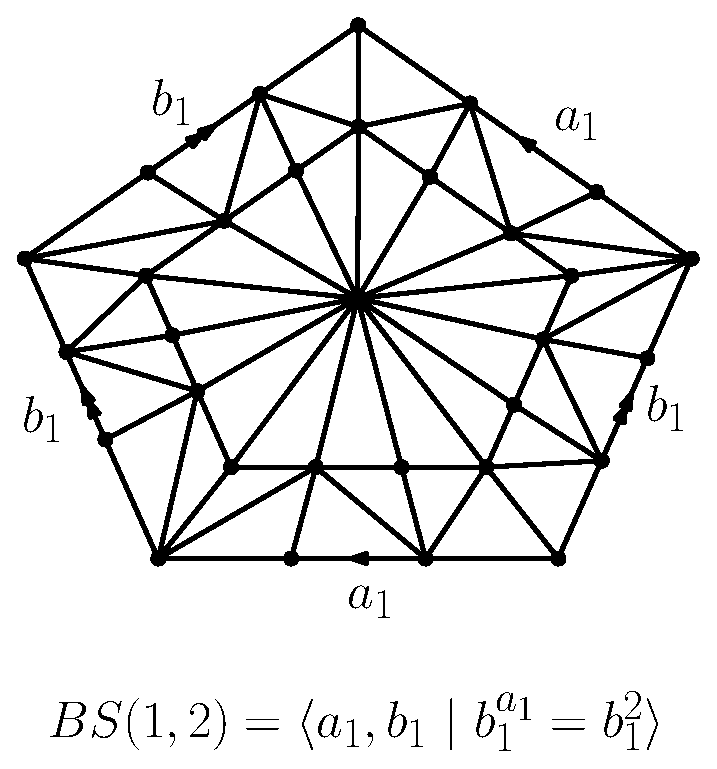
\includegraphics[scale=0.6]{BS}
\end{center}


Теперь возьмём 2 копии таких триангулированных пятиугольников и склеим из них $K(L, 1)$.


\begin{center}
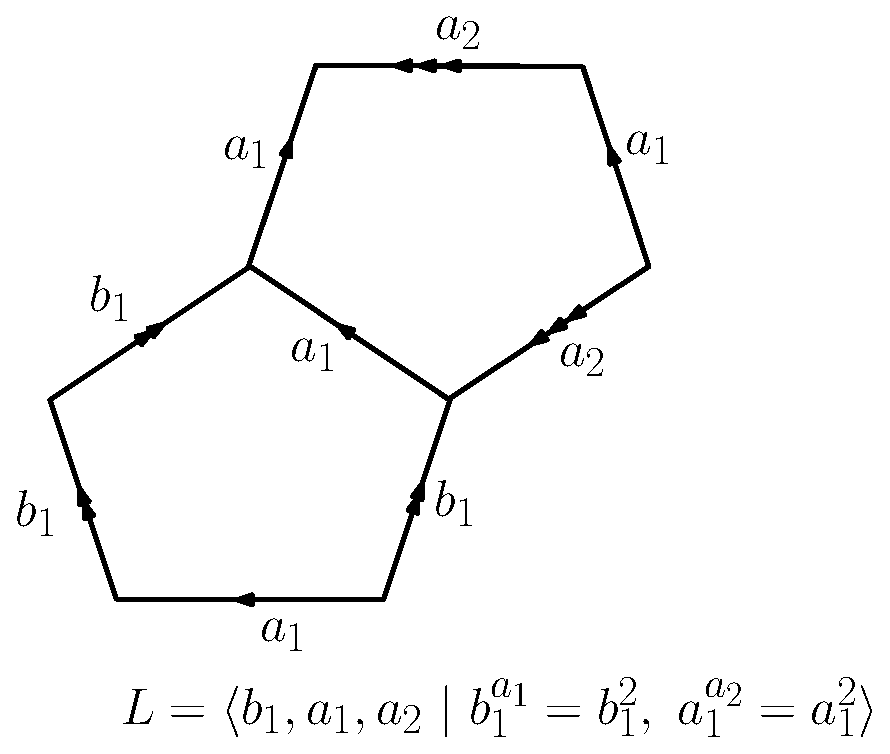
\includegraphics[scale=0.6]{L}
\end{center}


Наконец, возьмём 2 копии комплексов $K(L, 1)$ и склеим их.


\begin{center}
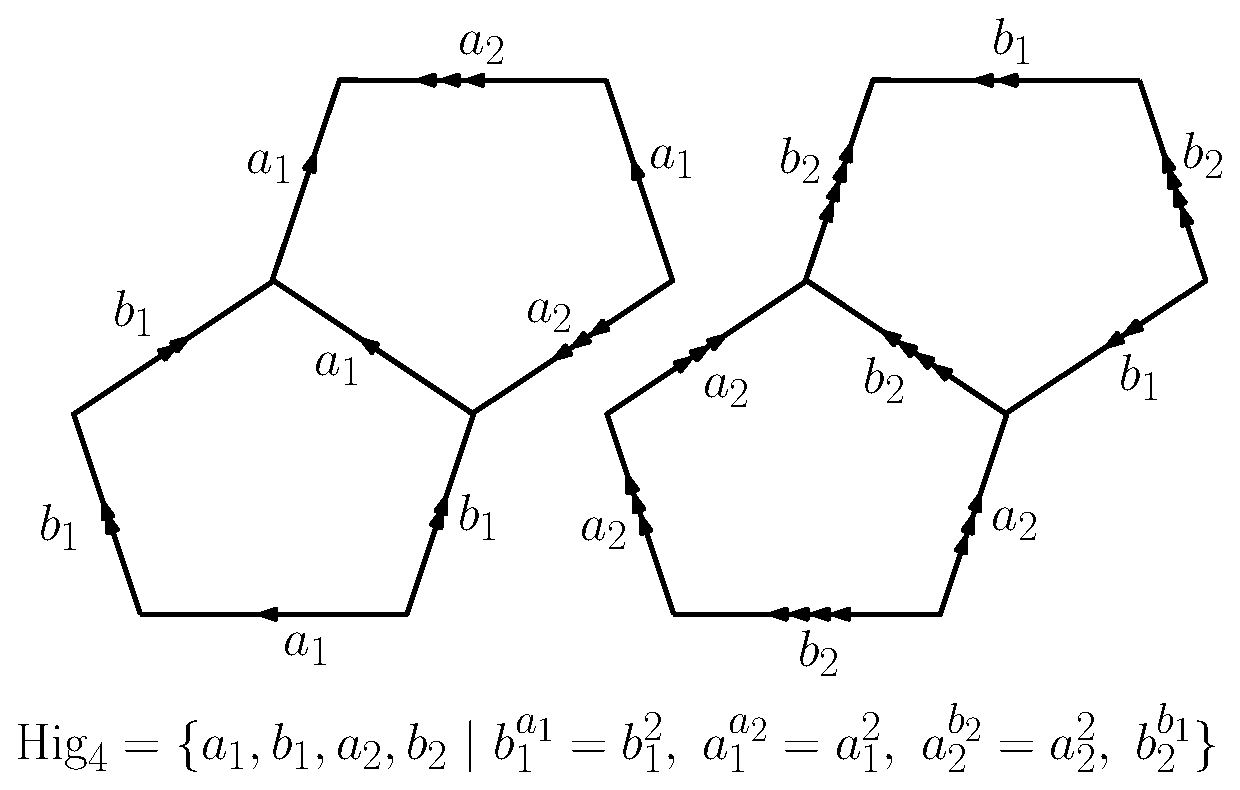
\includegraphics[scale=0.6]{Hig4}
\end{center}












\end{example} 











\section{Конструкция Кана-Тёрстона}




Д. Кан и У. Тёрстон получили (1976) следующий результат:

\begin{theorem}[Д. Кан, У. Тёрстон, 1976, \cite{Kan}]
Для любого линейно связного симплициального множества $X: \mathsf{sSet}_\ast$ с отмеченной точкой существует расслоение Серра $$t: TX\to X,$$ естественное по $X$ и обладающее следующими свойствами.

\begin{enumerate}[$($i$)$]
\item Естественное преобразование функторов $t: T\to \mathrm{Id}$ индуцирует изоморфизм групп сингулярных гомологий и когомологий с коэффициентами в произвольной локальной системе $\mathcal{A}$ на $X$, т. е. $$H_\ast(TX; t^\ast\mathcal{A})\cong H_\ast(X; \mathcal{A}),\ H^\ast(TX; t^\ast\mathcal{A})\cong H^\ast(X; \mathcal{A}).$$

\item Пространство $TX$ асферично, т. е. $TX\simeq K(G_X, 1)$, и отображение $t_\ast\pi_1: G_X \to \pi_1X$ --- эпиморфизм.

\item Ядро $P_X$ отображения $t_\ast\pi_1$ является совершенной нормальной подгруппой в $G_X$.

\item Гомотопический тип пространства $X$ полностью определяется парой групп $(G_X, P_X)$. А именно, пространство $X$ может быть получено с точностью до гомотопии применением к пространству $K(G_X, 1)$ функтора $(-)^+$ плюс-конструкции Квиллена относительно совершенной нормальной подгруппы $P_X$. Эквивалентно, $X$ может быть получено применением функтора послойного $\mathbb{Z}$-пополнения Боусфилда и Кана (см. [???]) к расслоению Серра $K(G_X, 1)\to K(G_X/P_X, 1)$.

\item Универсальное накрытие $\widetilde{X}$ над $X$ может быть получено с точностью до гомотопии применением функтора $\mathbb{Z}$-пополнения к $K(P_X, 1)$.

\item Ацикличный слой расслоения Серра $TX\to X$ получается с точностью до гомотопии применением функтора Дрора к $K(P_X, 1)$.    
\end{enumerate}
\end{theorem}



Приведём доказательства последних четырёх пунктов, поскольку они опущены в оригинальной статье Кана-Тёрстона.

\begin{proof} $(iii)$. Для точной последовательности $$1\to P_X\to G_X\to \pi_1X\to 1$$ имеет место спектральная последовательность Хохшильда-Серра $$H_p(\pi_1X; H_q(P_X; \mathbb{Z}))\rightarrow H_{p+q}(\pi_1X; \mathbb{Z}),$$ где $\mathbb{Z}$ --- тривиальный $\pi_1X$-модуль.

Запишем точную пятичленную последовательность $$H_2(\pi_1X)\to E^2_{2,0}\overset{d_{2}}{\to} E^2_{0, 1}\to H_1(\pi_1X)\to E^2_{1, 0}\to 0.$$ Имеем: $E^2_{2,0} = H_2(\pi_1X)$. Далее, $$E^2_{0,1} = H_0(\pi_1X; H_1(P_X)) = H_1(P_X)_{\pi_1X} = H_1(P_X),$$ поскольку индуцированное действие $\pi_1X$ на $\ker(G_X\to \pi_1X)$ тривиально. Наконец, $$E^2_{1,0} = H_1(\pi_1X; H_0(P_X)) = H_1(\pi_1X).$$ Из первого свойства функтора Кана-Тёрстона следует, что $H_2(G_X)\cong H_2(X)$, $H_1(G)\cong H_1(X)$. Кроме того, $H_1(\pi_1X)\cong H_1(X)$ (постоянные коэффициенты в $\mathbb{Z}$). Стало быть, мы получаем $$H_2(X)\twoheadrightarrow H_2(\pi_1X)\overset{0}{\to} H_1(P_X)\overset{0}{\to} H_1(G_X)\overset{\cong}{\to} H_1(X)\to 0.$$

Стрелка слева является эпиморфизмом в силу теоремы Хопфа. Значит, в силу сказанного выше, мы получаем, что $H_1(G_X) = 0$. 



$(iv)$. Покажем, что плюс-конструкция Квиллена однозначно с точностью до гомотопической эквивалентности, восстанавливает $X$ по $TX$ и совершенной нормальной подгруппе $P_X$ в $G_X = \pi_1(TX)$. Применим функтор Квиллена к отображению $t: TX\to X$, и мы получим отображение $$t^{+}: (TX, P_X)^{+}\to X.$$ Легко видеть, что отображение $t^{+}$ будет индуцировать изоморфизм на фундаментальных группах. Кроме того, по свойству плюс-конструкции мы будем также иметь и изоморфизм в любой системе локальных коэффициентов $\mathcal{A}$. Значит, по теореме Уайтхеда \ref{WhiteheadNonSimplyConnected} для неодносвязных пространств мы получаем, что $f$ --- гомотопическая эквивалентность.




Теперь докажем, что $X$ можно получить из $TX$ применением функтора $\mathbb{Z}_\infty$. Применив послойный функтор $\mathbb{Z}$-пополнения к расслоению Серра $TX\to X$, мы получим отображение $$f: \dot{\mathbb{Z}}_\infty TX\to X.$$ Покажем, что $f$ индуцирует гомотопическую эквивалентность. Для этого мы воспользуемся теоремой Уайтхеда \ref{WhiteheadNonSimplyConnected} для неодносвязного случая. Из рассмотрения точной последовательности расслоения $$\mathbb{Z}_\infty K(P_X,1)\to \dot{\mathbb{Z}}_\infty K(G_X, 1)\to K(\pi_1X, 1),$$ берущегося из основного свойства функтора послойного $\mathbb{Z}$-пополнения, получается, что $f$ индуцирует изоморфизм на фундаментальных группах $$f_\ast: \pi_1(\dot{\mathbb{Z}}_\infty K(G_X, 1))\cong \pi_1(X),$$ поскольку $\pi_1(\mathbb{Z}_\infty K(P_X, 1)) = 1$, см. \cite{Bousfield}.

\iffalse 

Последнее равенство имеет место в силу того, что $\pi_1(\mathbb{Z}_\infty K(P_X, 1))$ является групповым $\mathbb{Z}$-пополнением $(P_X)^{\widehat{}}_\mathbb{Z}$ группы $P_X$ и значит, совпадает с обратным пределом $$(P_X)^{\widehat{}}_{\mathbb{Z}} = \underleftarrow{\lim} \frac{P_X}{\lceil_n P_X} =  \underleftarrow{\lim} \{1\} = 1$$ где $\lceil_n P_X$ --- элемент нижнего центрального ряда для группы $P_X$, и последнее равенство имеет место в силу доказанной совершенности группы $P_X$. 

\fi

Рассмотрим морфизм расслоений Серра $$\xymatrix{
    K(P_X, 1) \ar[r] \ar[d] & K(G_X, 1) \ar[d] \ar[r] &  K(\pi_1X, 1) \ar@{=}[d] \\
    \mathbb{Z}_\infty K(P_X, 1) \ar[r]       & \dot{\mathbb{Z}}_\infty K(G, 1) \ar[r] &K(\pi_1X, 1) }$$ 
    
Этот морфизм индуцирует морфизм спектральных последовательностей Лере. Для доказательства того, что $f$ индуцирует изоморфизм в когомологиях с локальными коэффициентами, достаточно в силу теоремы Зимана показать, что для любой локальной системы $\mathcal{A}$ на $X$ $$H_\ast(K(P, 1); i^\ast\circ t^\ast\mathcal{A})\cong H_\ast(\mathbb{Z}_\infty K(P_X, 1); \mathbb{Z}_\infty i^\ast\circ \mathbb{Z}_\infty t^\ast\mathcal{A}),$$ где $i^\ast\circ t^\ast$ и $\mathbb{Z}_\infty i^\ast\circ \mathbb{Z}_\infty t^\ast$ являются композициями гомоморфизмов фундаментальных групп в данных расслоениях. Заметим, что эти композиции гомоморфизмов тривиальны, поэтому участвующие коэффициенты получаются тривиальными. Но $$H_\ast(\mathbb{Z}_\infty K(P_X, 1); \mathbb{Z})\cong H_\ast(K(P_X, 1); \mathbb{Z}),$$ поскольку пространство $K(P_X, 1)$ является $\mathbb{Z}$-хорошим в терминах работы Боусфилда и Кана. Последнее верно в силу совершенности группы $P_X$.


$(v)$. Этот пункт следует из предыдущего и точной последовательности расслоения $$\mathbb{Z}_\infty K(P_X,1)\to \dot{\mathbb{Z}}_\infty K(G_X, 1)\simeq X\to K(\pi_1X, 1).$$


$(vi)$. Мы имеем отображение $f: UX\to K(P_X, 1)$, где $UX$ является гомотопическим слоем расслоения Серра $TX\to X$. Применяя к $f$ функтор Дрора $A$ и учитывая, что $UX$ ациклично (это следует из спектральной последовательности Лере для данного расслоения и того, что $TX$ и $X$ имеют одинаковые гомологии), мы получаем отображение $$Af: UX\to AK(P_X, 1).$$ Очевидно, $Af$ индуцирует изоморфизм в гомологиях между полученными ацикличными пространствами. Из свойства функтора Дрора следует, что $\pi_1(AK(P_X, 1))$ $= \pi_1(AP_1K(P_X, 1)) = N,$ где $P_1(P_X)$ --- первый этаж системы Постникова пространства $K(P_X, 1)$, а $N$ --- максимальная совершенная подгруппа в группе $P_X$, т. е. $N = P_X$. Кроме того, $\pi_1(UX)\cong P_X$ из точной последовательности расслоения выше. Значит, $f$ индуцирует изоморфизм и на фундаментальных группах. Дальнейшее следует из теоремы Уайтхеда.




\end{proof}





\subsection{Пример: случай сфер}

Для конкретного случая сфер $\mathbb{S}^n$ построим явно пространство $T\mathbb{S}^n$ типа $K(\pi, 1)$ и отображение $$t: T\mathbb{S}^n\to \mathbb{S}^n,$$ такие, что на (ко)гомологиях индуцируются изоморфизмы. В этом параграфе мы следуем статье \cite{BDH}.

\subsubsection{Двумерная сфера}

Пусть вначале мы имели пространство $X=\mathbb{S}^1$. Мы хотим получить из него пространство типа $K(\pi, 1)$, которое бы имело те же гомологии, что и $\mathbb{S}^2$. 

Возьмём в качестве группового конуса $C\mathbb{Z}$ группу Хигмана $\mathrm{Hig}_4$. Это вложение индуцирует отображение $$\mathbb{S}^1\simeq K(\mathbb{Z}, 1)\to K(\Hig_4, 1)\eqno (\star)$$ Склеив две копии цилиндра отображения $(\star)$ вдоль окружности, мы получим согласно утверждению \ref{wh} искомое пространство $$K(\Hig_4\star_{\mathbb{Z}}\Hig_4, 1).$$ На построенном пространстве можно ввести структуру 2-мерного симплициального комплекса, взяв в качестве $K(\Hig_4, 1)$, например, триангуляцию, построенную ранее. Для построения отображения $$t: K(\Hig_4\star_{\mathbb{Z}}\Hig_4, 1)\to \mathbb{S}^2$$ отправим каждый цилиндр в треугольник так, чтобы 2-мерный симплициальный комплекс $K(\mathrm{Hig}_4, 1)$ отправился в барицентр этого треугольника, а на исходной окружности возьмём $t$ тождественным.


\subsubsection{$n$-мерная сфера}

После построения пространства $T\mathbb{S}^2$ можно продолжить процесс, используя следующую теорему

\begin{theorem}
Пусть имеется вложение $F\to G$, где $G$ --- ацикличная. Тогда амальгама $G\star_F G$ вкладывается в ацикличную группу $$(A\times F)\star_F G$$ где $A$ --- любая нетривиальная ацикличная группа.
\end{theorem}

Эта замечательная теорема позволяет нам продолжить индуктивное построение пространств $T\mathbb{S}^n$.

Пусть $n=3$. Возьмём в качестве гомоморфизма в лемме отображение $\mathbb{Z}\hookrightarrow \Hig_4$. Тогда мы будем иметь вложение в ацикличную группу $$\Hig_4\star_\mathbb{Z}\Hig_4\hookrightarrow (\Hig_4\times \mathbb{Z})\star_{\mathbb{Z}}\Hig_4$$ и снова образуем при помощи таких вложений гомологическую надстройку: $$T\mathbb{S}^3 = \left [ (\Hig_4\times \mathbb{Z})\star_{\mathbb{Z}}\Hig_4 \right ] \underset{\Hig_{4}\star_{\mathbb{Z}}\Hig_{4}}{\star} \left [ (\Hig_4\times \mathbb{Z})\star_{\mathbb{Z}}\Hig_4 \right ]$$

Теперь на каждом следующем шаге $n$ будем брать в качестве вложения $F\to G$ из леммы вложение групп из предыдущего шага $n-1$.  

Причём для каждого $n$ будет получаться $n$-мерный конечный симплициальный комплекс по утверждению \ref{finite}, в силу того, что геометрическая размерность группы Хигмана равна 2, а группы $\mathbb{Z}$ --- равна 1. 











\section{Метод Маундера построения пространства Кана-Тёрстона}

Изложим здесь довольно простое доказательство части утверждений теоремы Кана-Тёрстона, найденное Маундером в \cite{Maunder}.

\begin{theorem}[Д. Кан, У. Тёрстон, 1976, \cite{Kan}]
Для каждого линейно связного пространства $X$ с отмеченной точкой существует пространство $TX$ и отображение $$TX\overset{t}{\to} X,$$ естественное по $X$ и обладающее свойствами:
\begin{enumerate}[\bf 1.]
\item Отображение $t$ индуцирует изоморфизм в (сингулярных) гомологиях и когомологиях $$H_\bullet(TX; t^\ast \mathcal{A})\cong H_\bullet(X; \mathcal{A})$$ для любой локальной системы коэффициентов $\mathcal{A}$ на $X$; 

\item $\pi_i(TX)$ тривиальна для $i\neq 1$, и отображение на фундаментальных группах $\pi_1t$ --- эпиморфизм;

\item Если исходным пространством был конечный симплициальный комплекс $X$, то $TX$ может быть выбрано конечным.
\end{enumerate}
\end{theorem}

\begin{proof}[Доказательство {\normalfont (C. R. F. Maunder, 1981, \cite{Maunder})}]

Сначала докажем утверждение для конечных симплициальных комплексов индукцией по числу  сиплексов. Пусть для любого комплекса $L$ с не более, чем $N-1$ симплексами отображение $t:TL\to L$ удовлетворяет пунктам теоремы. Предположим также, что на подкомплексах $M\subset L, TM=t^{-1}M$, и $\pi_1(TM)\to \pi_1(TL)$ является инъекцией. Поскольку всякий 1-мерный комплекс является пространством типа $K(\pi, 1)$, то отображение $t$ может быть выбрано тождественным, если $\dim L\leqslant 1$.

Пусть теперь $K$ получается из $L$ приклеиваением $n$-симплекса $\sigma$ к $\partial\sigma\subset L$, где $\dim \sigma\geqslant 2$. Тогда $T(\partial\sigma)$ является подпространством $TL$, и если $f:\sigma\to \Delta^n$ --- симплициальный гомеоморфизм на стандартный $n$-симплекс, то отображение $Tf:T(\partial\sigma)\to T(\partial\Delta^n)$ является гомеоморфизмом. Кроме того, $T(\partial\Delta^n)$ является пространством типа $K(\pi, 1)$ по предположению индукции. 

Вложение группы $\pi$ в ацикличное пространство $C\pi$ индуцирует отображение классифицирующих пространств $g: T(\partial \Delta^n)\to K(C\pi, 1)$. 

Тогда можно приклеить цилиндр отображения $g\circ Tf$ вдоль $T(\partial\sigma)$ к $TL$, а отображение $t$ можно продолжить до отображения $t:TK\to K$, отправляя $K(C\pi, 1)$ в барицентр симплекса $\sigma$.

Проверим теперь, что отображение $t:TK\to K$ --- искомое:

\begin{enumerate}[\bf 1.]

\item Рассмотрим две точные последовательности Майера-Виеториса для пространства $$TK=\mathrm{Cyl}(g\circ Tf)\sqcup_{T(\partial\sigma)}TL$$ и для пространства $$K=\sigma\sqcup_{\partial \sigma}L.$$ Тогда по предположению индукции и по 5-лемме мы будем иметь изоморфизм $H_n(TK; A)\cong H_n(K; A)$.

\item  Склеиваемые пространства являются асферичными и склейка происходит вдоль асферичного пространства, также в фундаментальные группы пространств $TL$ и $K(C\pi, 1)$ вкладывается группа $\pi$, поэтому по теореме Уайтхеда пространство $TK=\mathrm{Cyl}(g\circ Tf)\sqcup_{T(\partial\sigma)}TL$ будет иметь тип $K(\pi_1(TK), 1)$, где $\pi_1(TK)=\pi_1(TL)\star_{\pi} C\pi$. Кроме того, отображение $t_\star: \pi_1(TK)\to \pi_1(K)$ является эпиморфизмом, поскольку $\pi_1(K)=\pi_1(L)\star_{\pi_1(\partial\sigma)}\pi_1(\sigma)$ и в силу предположения индукции. 

\end{enumerate}

Заметим, что конструкция пространства $TK$ является естественной относительно симплициальных отображений, сохраняющих строгий порядок. Таким образом, для конечных симплициальных комплексов теорема доказана. Беря копредел по конечным подкомплексам, можно получить результат для бесконечных сиплициальных комплексов.

В общем случае, если $X$ --- произвольное линейно связное пространство, мы можем положить $$TX=T(|SX|''),$$ где $SX$ --- сингулярный комплекс, рассматриваемый, как симплициальное множество, $|\cdot|$ --- реализация симплициального множества, а двойной штрих --- второе барицентрическое подразделение. Эта конструкция также является естественной.

Докажем последний пункт теоремы. Пусть изначально $X$ было конечным симплициальным комплексом. 

Будем строить индукцией по размерности и числу клеток пару конечных симплициальных пространств $(UK, TK)$ и отображение пар $t: (UK, TK) \to (CK, K)$, где $CK$ --- конус над $K$, такое, что ограничение $t$ на $TK$ является искомым отображением. Предположим, что мы уже построили $t: (UL, TL) \to (CL, L)$, такое, что 

\begin{enumerate}[(i)]

\item $(UL, TL)$ является конечной симплициальной парой, $\dim UL = n+1$, $\dim TL = n$;

\item Для любого связного $r$-мерного подкомплекса $M$ комплекса $L$ выполнено: $t^{-1}(CM)$ и $t^{-1}(M)$ являются $(r+1)$- и $r$-мерными подкомплексами $UL$ и  $TL$ соответственно, ограничения $t: t^{-1}(CM)\to CM$, $t: t^{-1}(M)\to M$ удовлетворяют первым двум условиям теоремы. Более того, пусть $\pi_1t^{-1}(CM)\to \pi_1UL$, $\pi_1t^{-1}(M)\to \pi_1TL$ и $\pi_1t^{-1}(M)\to\pi_1t^{-1}(CM)$ являются инъекциями. 

\end{enumerate}    


База индукции --- нульмерный остов. На нём полагаем $t$ тождественным отображением, $UL = CL$. Теперь пусть $K$ получен приклейкой симплекса $\sigma$, размерности $n\geqslant 1$. Тогда по предположению индукции $t^{-1}(C\partial\sigma)$ и $t^{-1}(\partial\sigma)$ являются подкомплексами $UL$ и $TL$ соответственно. Пусть $TK$ получается из $TL$ приклейкой копии $t^{-1}(C\partial \sigma)$ вдоль $t^{-1}(\partial\sigma)$. Продолжение $t: TK\to K$ будет отправлять $t^{-1}(C\partial \sigma)$ в $C\partial\sigma$, причём $C\partial\sigma$ отождествляется с $\sigma$ так, что вершина симплекса $C\partial\sigma$ идёт в барицентр $\hat{\sigma}$ симплекса $\sigma$ (а дальше отображение продолжается по линейности). Для построения $UK$ рассмотрим комплекс $$X = t^{-1}(C\partial\sigma)\sqcup_{t^{-1}(\partial\sigma)}t^{-1}(C\partial\sigma).$$ Тогда $X$ будет пространством типа $K(\pi, 1)$, где $\pi = G\star_F G$, $G = \pi_1(t^{-1}(C\partial\sigma))$ и ясно, что $\dim X = \dim \sigma = n$. Рассмотрим следующее образование: $$UK := (UL\cup TK)\sqcup_X \mathrm{Cyl},$$ где $\mathrm{Cyl}$ --- это цилиндр отображения $X = K(G\star_F G, 1)\to K((A\times F)\star_F G, 1)$, в котором $A$ --- нетривиальная геометрически конечная ацикличная группа с $\dim K(A, 1) = 2$ (например, группа Хигмана $\Hig_4$). Отображение $t$ продолжается на $UK$ отправлением $K((A\times F)\star_F G, 1)$ в барицентр конуса $C\sigma$. Если $\dim\sigma = 1$, нужно вместо $G\star_F G$ взять группу $\mathbb{Z}$, которая должна вкладываться в $A$ вместо $(A\times F)\star_F G$.

Пространство $K((A\times F)\star_FG, 1)$ является ацикличным относительно системы коэффициентов $t^\ast\mathcal{A}$, поскольку последняя тривиальна. Действительно, она получается из системы $\mathcal{A}$ на $X$ pullback'ом вдоль отображения $t: t^{-1}(C\partial\sigma)\to C\partial\sigma$, но конус $C\partial\sigma$ стягиваем, и значит, система $\mathcal{A}$ на нём тривиальна. 

Далее, из доказательства утверждения [??] получается, что $\dim K((A\times F)\star_FG, 1) = n + 1$.   

Заметим, что на каждом шаге цилиндры отображения можно представить в виде симплициального разбиения, поэтому мы получаем конечный симплициальный комплекс с требеумыми свойствами. Эта конструкция также естественна по пространству $X$.  


\end{proof}


\begin{example}
Приведём здесь пошаговое построение конструкции Маундера пространства Кана-Тёрстона для 2-мерного диска $\mathbb{D}^2$.

{\bf Шаг 0.} Сначала мы имели нульмерный остов, состоящий из 3 вершин $L = \{[0], [1],  [2]\}$. В этом случае конус является объединением трёх отрезков: $CL = \{ [3, 0], [3, 1], [3, 2] \}$. Конструкция Кана-Тёрстона $TL$ совпадёт с $L$ и пространство $UL$ совпадёт с $CL$. Отображение пар $t: (UL, TL) \to (CL, L)$ будет тождественным.

{\bf Шаг 1.} Приклеим 1-симплекс $\sigma = [0, 1]$ к комплексу $L$ и получим комплекс $K$. Тогда $C\partial \sigma$ будет <<рогом>> $[3, 0]\cup [3, 1]$, $t^{-1}(C\partial \sigma) = [3, 0]\cup [3, 1]$, и $t^{-1}(\partial\sigma) = [0]\cup [1]$. Значит, $TK = TL\sqcup_{t^{-1}(\partial\sigma)} t^{-1}(C\partial\sigma) = [3', 0]\cup[3', 1]\cup [2]$ --- это объединение двух отрезков и точки, причём при отображении $t: TK\to K$ вершина $[3]$ отображается в середину отрезка $[0, 1]$. 

\begin{center}
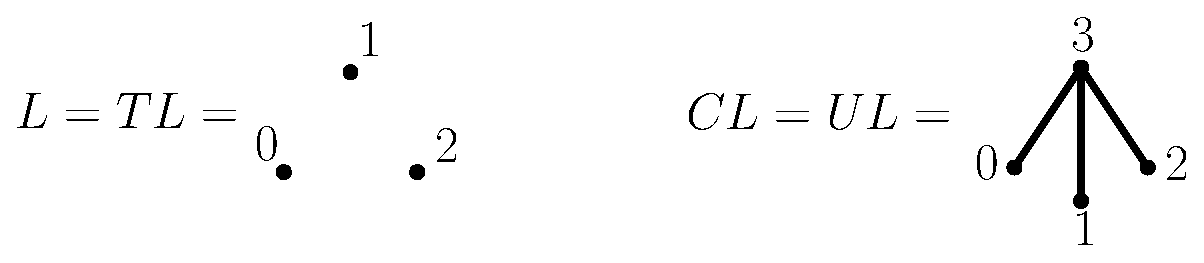
\includegraphics[scale=0.5]{pict1}
\end{center}


Пространство $X = t^{-1}(C\partial\sigma)\sqcup_{t^{-1}(\partial\sigma)} t^{-1}(C\partial\sigma) = [3, 0]\cup [3,1] \cup [3', 0] \cup [3', 1]$ --- это окружность $K(\mathbb{Z}, 1)$. 

\begin{center}
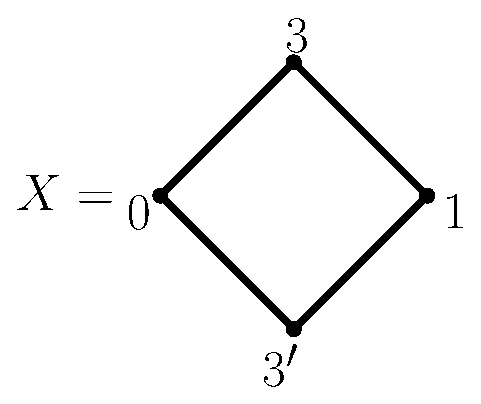
\includegraphics[scale=0.5]{pict2}
\end{center}


Далее, мы должны приклеить к объединение $UL\cup TK$ к пространству $X$. В результате получится: 


\begin{center}
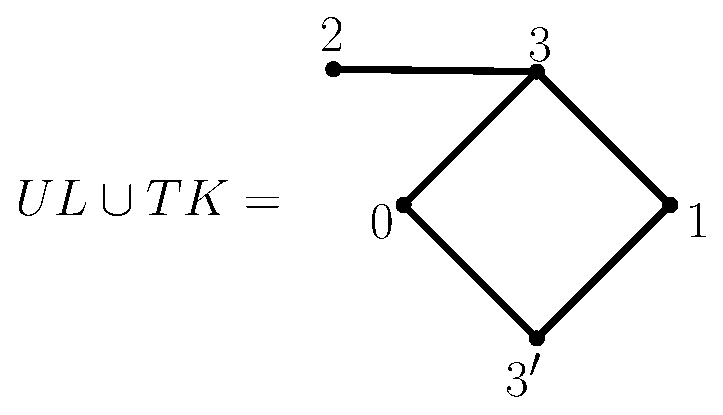
\includegraphics[scale=0.5]{pict3}
\end{center}

Комплекс $CK$ будет выглядеть так:

\begin{center}
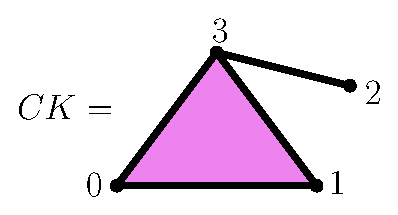
\includegraphics[scale=0.8]{pict8}
\end{center}


Теперь нужно приклеить к пространству $UL\cup TK$ цилиндр отображения $X\simeq K(\mathbb{Z}, 1)\to K(\mathrm{Hig}_4, 1)$, и мы получим пространство $UK$. 

Отображение $t: TK\to K$ будет отображать комплекс $K(\Hig_4, 1)$ в барицентр $[4]$ треугольника $[0, 3, 1]$. При этом грани <<призмы>>, примыкающие к сторонам $[3, 0]$ и $[3, 1]$ отобразятся на треугольник $[4, 0, 1]$. Две другие грани <<призмы>>, примыкающие к отрезкам $[0, 3]$ и $[3, 1]$ отобразятся на треугольники $[4, 0, 3]$ и $[4, 3, 1]$ соответсвенно.  

Обозначим для удобства дальнейшего изложения получившееся образование за $A:=UK$. 


\begin{center}
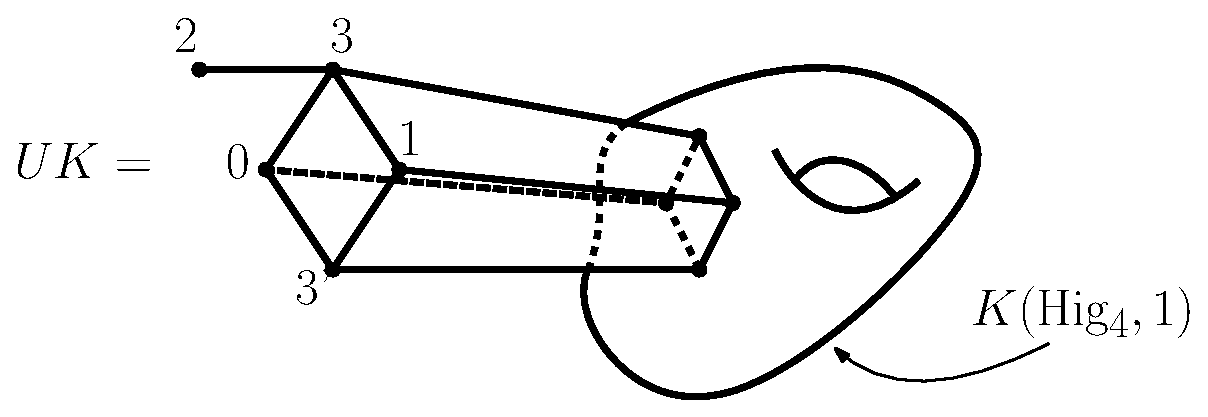
\includegraphics[scale=0.5]{pict4}
\end{center}





{\bf Шаг 2.} Переобозначим полученную пару комплексов через $(UL, TL)$ и будем приклеивать следующий 1-симплекс $[1, 2]$.

Пока мы имеем такие данные:   

\begin{center}
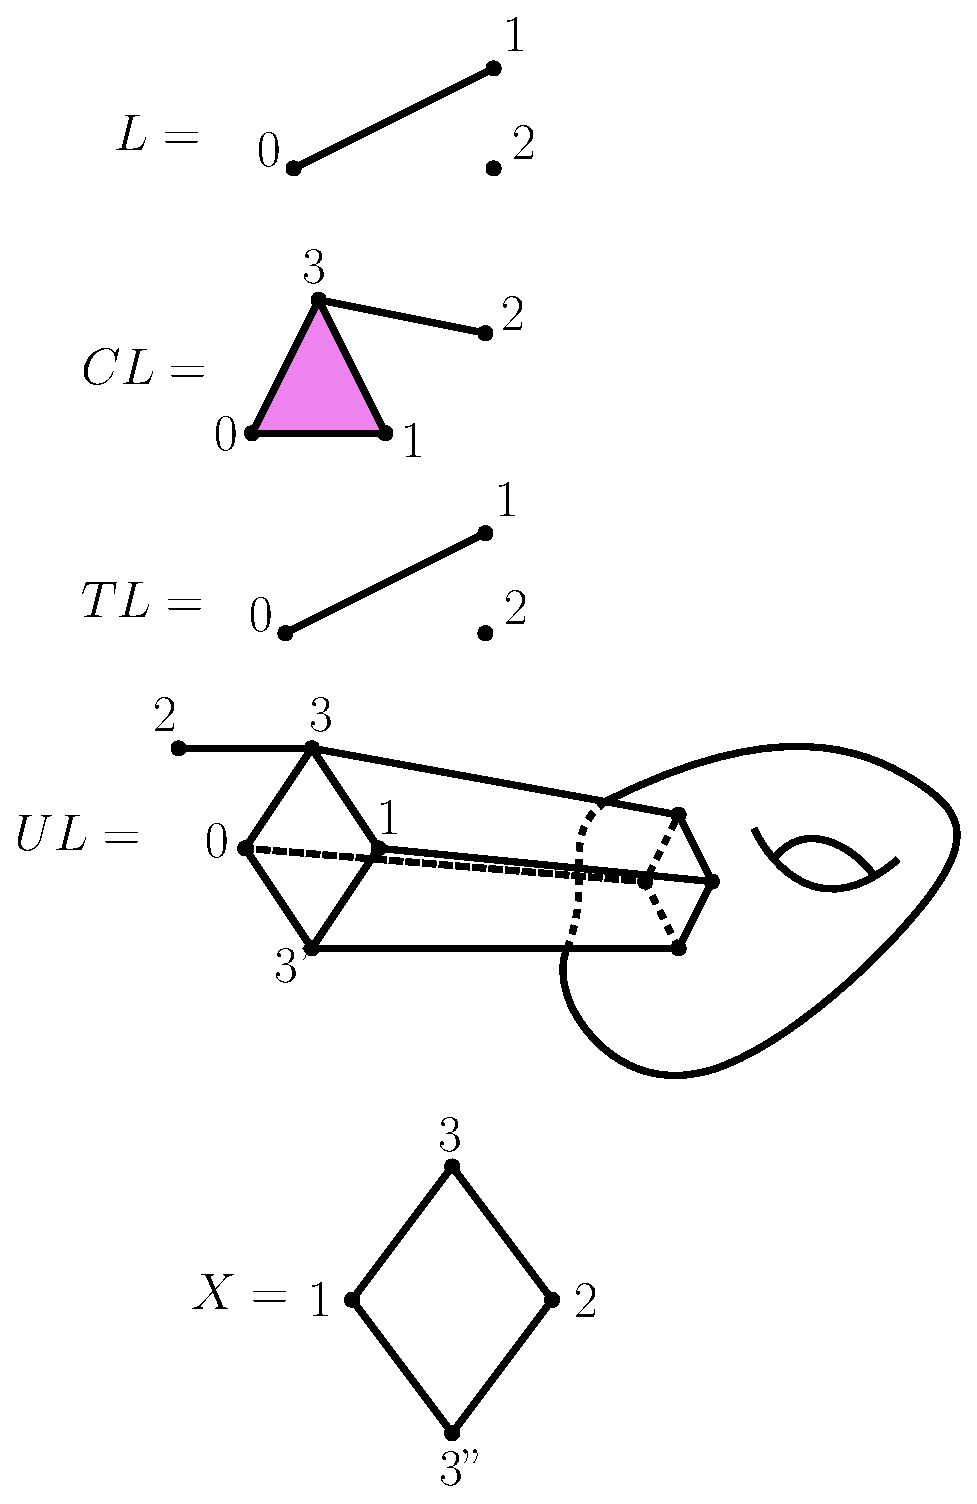
\includegraphics[scale=0.4]{pict5}
\end{center}
 

Пространство $TK$ будет представлять собою $[0, 1]\cup [3'', 1]\cup [3'', 2]$ и будет отображаться в $K$, отправляя точку $3''$ в барицентр отрезка $[1, 2]$. В качестве пространства $UK$ будет выступать объединение отрезка $[0, 1]$ и пространства с двумя склеенными копиями $A$, причём вторая копия $A$ будет подклеиваться к <<рогу>> $[3,2]\cup [3, 1]$. 

{\bf Шаг 3.} Приклеим третье ребро $[0, 2]$. В результате, к $UL$ подклеится ещё одна копия пространства типа $A$ с прошлого шага, но уже к рогу $[3, 2]\cup [3, 0]$, также к $UL$ подклеится отрезок $[1, 2]$. Пространство Кана-Тёрстона будет $[0, 1]\cup [1, 2]\cup [3''', 2]\cup [3''', 0]$ --- окружность.



{\bf Шаг 4.} Подклейка двумерной клетки к границе треугольника. Комплекс $T\Delta^2$ будет представлять собой три образования типа $A$, склеенных вдоль трёх рогов с общей вершиной $[3]$ и остальными вершинами $[0], [1], [2]$. Приведём здесь схему расположения <<рогов>>:


\begin{center}
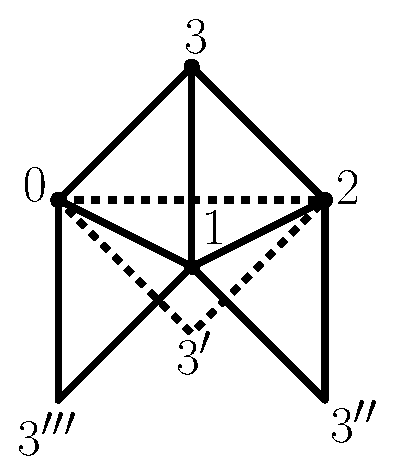
\includegraphics[scale=0.5]{pict7}
\end{center}

Как устроено отображение $t: TK\to K$? Конус над границей треугольника $[0, 1, 2]$ с вершиной $[3]$ переходит в треугольник $[0, 1, 2]$ так, что вершина $[3]$ отображается в барицентр треугольника $[0, 1, 2]$, а остальные вершины конуса переходят тождественно в вершины этого треугольника. На другие точки этого конуса отображение $t$ продолжается по линейности. На каждом из трёх подклееных цилиндров отображение $t$ уже задано.    
 
Полученное пространство $T\mathbb{D}^2$ имеет в качестве фундаментальной группы свободное произведение трёх групп Хигмана $\Hig_4$. То есть для стягиваемых пространств конструкция Маундера даёт нестягиваемые ацикличные пространства. Это наглядно иллюстрирует тот факт, что функтор Кана-Тёрстона не является гомотопическим.








\end{example}






\subsection{Важное следствие: эквивалентность категорий}


В работе \cite{Kan} Кана и Тёрстона утверждается, что в конструкции возможно и обратное построение. А именно, исходное пространство $X$ может быть восстановлено с точностью до гомотопии из пары $(G_X, P_X)$ при помощи плюс-конструкции Квиллена, где $G_X = \pi_1(TX)$, $P_X = \ker \pi_1 t X$ --- нормальная совершенная подгруппа $G_X$. То есть $X = (G_X, P_X)^+$.

Напомним здесь вкратце плюс-конструкцию Квиллена. Она позволяет по данному комплексу $X$ и данной совершенной нормальной подгруппе $P$ фундаментальной группы $\pi_1(X)$ строить комплекс $X^+$ с теми же гомологиями и с убитой подгруппой $P$ в фундаментальной группе. 

А именно, существует пространство $X^+$ и отображение $i:X\to X^+$, для которых 

\begin{enumerate}[i)]

\item имеет место точная последовательность $$1\to P\to \pi_1(X)\overset{i_{\star}}{\to} \pi_1(X^+)\to 1;$$

\item если группа $\pi_1(X^+)$ действует на коммутативной группе $A$, то для локальной системы $\mathcal{A}$ над $X^+$  и индуцированной системы $\mathcal{A}^\ast$ над $X$ гомоморфизм $i^\ast:H^\ast(X^+; \mathcal{A})\to H^\ast(X; \mathcal{A}^\ast)$ является изоморфизмом.

\begin{corollary}[Д. Кан, У. Тёрстон, \cite{Kan}]

Имеет место эквивалентность категорий $$\Ho \mathscr{CW}\cong \mathscr{GP}[\Gamma^{-1}]$$ 

Здесь категория $\Ho\mathscr{CW}$ состоит из $CW$-комплексов и классов гомотопий отображений между пространствами. Объектами категории $\mathscr{GP}$ служат пары дискретных групп $(G, P)$, где $P$ --- совершенная нормальная подгруппа $G$, отображения --- гомоморфизмы $f:(G, P)\to (G', P')$, для которых $f(P)\subset P'$, $\Gamma$ состоит из тех морфизмов $f:(G, P)\to (G', P')$ из $\mathrm{Mor}(\mathscr{GP})$, что $f: G/P\cong G'/P'$ и $f_\ast: H_\ast(G; A)\cong H_\ast (G'; A)$ для любого $G'/P'$-модуля $A$.
\end{corollary} 




\begin{proof}[Схема доказательства \cite{Deleanu}]
Эта эквивалентность следует из того, что конструкция Кана-Тёрстона <<обратна>> плюс-конструкции Квиллена. Имеется следующая диаграмма категорий и функторов между ними:

$$\Ho\mathscr{CW}\stackrel[\Ho()^{+}]{\Ho J}{\rightleftarrows}\Ho\mathscr{XP}\overset{\Ho}{\leftarrow}\mathscr{XP}\stackrel[I]{T}{\rightleftarrows}\mathscr{\mathscr{AP}}\overset{\Ho}{\rightarrow}\Ho\mathscr{AP}\stackrel[B]{\pi}{\rightleftarrows}\mathscr{GP}$$

Здесь

\begin{itemize}
\item  $\mathscr{XP}$ --- категория пар $(X, P)$, $P\vartriangleleft \pi_1(X)$, $P$ совершенна

 \item $\mathscr{AP}$ категория пар $(X, P)$, $P\vartriangleleft \pi_1(X)$, $X$ асферично, $P$ совершенна 

\item $\mathscr{GP}$ --- категория пар $(G, P)$, $P\vartriangleleft G$, $P$ совершенна

\end{itemize}

Переходом к подходящим локализациям можно добиться того, чтобы все стрелки в диаграмме стали обратимыми, и тогда мы получим цепочку эквивалентностей категорий, из которой будет следовать требуемое.
\end{proof}







\end{enumerate}








\section{Группы, свободно действующие на ацикличных пространствах}


Рассмотренные выше функторы дают надежду на обобщение понятия универсального расслоения. А именно, для данной группы $G$ зададимся поиском ацикличного, но не стягиваемого пространства $\mathcal{E}G$, на котором дискретная группа $G$ действует свободно.

Естественность функтора Дрора давала надежду на то, что он переводит накрытия симплициальных множеств в накрытия. Другая гипотеза состояла в том, что композиция $A\widetilde{X}\to \widetilde{X}\to X$ является накрытием.  

Однако обе эти гипотезы неверны, поскольку имеет место следующее

\begin{statement}
Если $\mathcal{E}G\to \mathcal{B}G$ --- $G$-накрытие с гомологически тривиальным $\mathcal{E}G$, то $\mathcal{B}G$ имеет такие же гомологии с коэффициентами в тривиальном $G$-модуле $\mathbb{Z}$, как и $BG$.
\end{statement}

\begin{proof}
Рассмотрим спектральную последовательность Картана-Лере $$H_p(G; H_q(\mathcal{E}G))\Rightarrow H_\ast(\mathcal{B}G).$$ Она вырождается во втором члене, поэтому $$H_n(\mathcal{B}G)\cong H_n(G; H_0(\mathcal{E}G)) = H_n(G; \mathbb{Z}) = H_n(G).$$ Последнее равенство верно в силу тривиальности $G$-модуля $\mathbb{Z}$.
\end{proof}

После чего возникла третья гипотеза, связанная уже с применением функтора Кана-Тёрстона: если $\widetilde{X}\to X$ является универсальным $G$-накрытием, то $T\widetilde{X}\to TX$ является $G$-накрытием.










\section{Классифицирующие пространства моноидов}

Как мы знаем, по любой дискретной группе $G$ можно построить классифицирующее пространство $BG$, рассмотрев бар-конструкцию. 

Но можно построить $BG$ как реализацию нерва некоторой категории. А именно, пусть $\mathscr{G}$ --- категория, состоящая из одного объекта и морфизмов, соответствующих элементам группы $G$. Нервом категории $\mathscr{G}$ будет являться симплициальное множество, $n$-симплекс которого являет собой последовательность $$\bullet \stackrel{g_{1}}{\to} \bullet \stackrel{g_{2}}{\to} \bullet\to ... \to \bullet \stackrel{g_{n}}{\to}\bullet$$ Оператор грани $d_i$ будет сопоставлять данной последовательности следующую: $$\bullet \stackrel{g_{1}}{\to}\bullet\to...\to \bullet \stackrel{g_{i+1}g_i}{\to}\bullet\to  ...\to \bullet \stackrel{g_{n}}{\to}\bullet$$ Отображение вырождения $s_i$ будет вставлять на место $i$ тождественный морфизм, соответствующий единице группы.

\begin{proposition}
Бар-конструкция для $G$ и геометрическая реализация нерва $|\mathcal{N}(\mathscr{G})|$ построенной выше категории $\mathscr{G}$ гомеоморфны.
\end{proposition} 

Симплициальную конструкцию классифицирующего пространства безболезненно можно перенести на случай любого моноида $M$. Но в этом случае не следует ожидать, что $BM$ будет слабо гомотопически эквивалентно пространству $K(G, 1)$, где $G$ --- некоторая дискретная группа. Это следует из такого замечательного результата:

\begin{theorem}[D. McDuff, 1978, \cite{McDuff}]
Любое линейно связное пространство слабо гомотопически эквивалентно классифицирующему пространству $BM$ некоторого дискретного моноида $M$. 
\end{theorem}

Можно задаться вопросом о том, в каких случаях всё же $BM\simeq K(G, 1)$. Естественно ожидать, чтобы группа $G$ была в некотором смысле близка к исходному моноиду $M$. Для любого моноида можно построить такую универсальную группу $G$, и она называется {\it группофикацией} моноида $M$. Рассмотрим свободную группу $\Gamma$, натянутую на элементы моноида $M$ и формально обратные к ним и профакторизуем $\Gamma$ по наименьшей нормальной подгруппе $N$, содержащей соотношения вида $xy=z$, если такое равенство имело место в исходном моноиде $M$. Тогда $\Gamma/N$ называется группофикацией моноида $M$.

\begin{defi}

Группофикацией моноида $M$ называется такая группа $G$ с гомомоморфизмом $\varphi$, что для любой группы $H$ и любого гомоморфизма $\psi: G\to H$ существует единственный гомоморфизм $f:M\to H$, замыкающий диаграмму до коммутативной: 

$$
\xymatrix{
    M  \ar[dr]_f \ar[r]^\varphi & G \ar@{-->}[d]^\psi \\
                         & H }
$$

\end{defi}

 



\begin{example}[А. Мальцев, 1937, \cite{Malcev}, \cite{Lenz}]

Рассмотрим свободный моноид $$F=\langle a, b, c, d, x, y, u, v \rangle$$ и его фактор $\mathcal{M}$ по отождествлениям $(ax, by),\ (cx, dy)$ и $(au, bv)$. Мальцев показал, что $cu\neq dv$ и что моноид $\mathcal{M}$ несокращаемый. Откуда получается, что $\mathcal{M}$ нельзя вложить ни в какую группу, иначе было бы: $[d^{-1}c]=[yx^{-1}]=[b^{-1}a]=[vu^{-1}]$. Значит, $[cu]=[dv]$ 

\end{example} 



Этот пример показывает, что не всегда моноид вкладывается в свою группофикацию. Однако в некоторых случаях вложение имеет место:

\begin{statement}
Отображение в группофикацию коммутативного сокращаемого моноида является вложением.
\end{statement}

Здесь под {\it сокращаемым моноидом} понимается такой моноид $M$, в котором из $xy=xz$ следует, что $y=z$ и из $yx=zx$ следует, что $y=z$.






\iffalse

\section{Связь с торической топологией}


В торической топологии известно расслоение полиэдральных произведений



\begin{theorem}[\cite{Toric}]
Для любого симплициального комплекса $\mathcal{K}$ на $[m]$ имеется расслоение $$(P\bm{X}, \Omega\bm{X})^\mathcal{K}\to (\bm{X}, \mathrm{pt})^\mathcal{K}\to (\bm{X}, \bm{X})^\mathcal{K}.$$
\end{theorem}


Здесь $(\bm{X}, \bm{A})=\{ (X_1, A_1), ..., (X_m, A_m) \}$, $A_i\subset X_i$. Для каждого симплекса $I\subset \mathcal{K}$ определим $$(\bm{X}, \bm{A})^I=\left \{(x_1, ..., x_m)\in \prod\limits_{j=1}^m X_j: x_j\in A_j,\text{если $j\notin I$} \right \}.$$ Тогда {\it полиэдральным произведением} называется

$$(\bm{X}, \bm{A})^\mathcal{K}=\bigcup\limits_{I\in \mathcal{K}}(\bm{X}, \bm{A})^I=\bigcup\limits_{I\in \mathcal{K}}\left ( \prod\limits_{i\in I} X_i\times \prod\limits_{i\neq I} A_i   \right )$$

Если в этом расслоении положить $X=B \mathbb{S}^1=\mathbb{C}P^\infty$, то получится классическое расслоение со слоем, являющимся момент-угол комплексом $$\mathcal{Z}_{\mathcal{K}}\to (\mathbb{C}P^\infty, \mathrm{pt})^{\mathcal{K}}\to (\mathbb{C}P^\infty)^m$$

В случае, когда семейство $\bm{X}$ состоит из одинаковых пространств $X$ будем во всех полиэдральных произведениях писать $X$ вместо $\bm{X}$.




Мы хотим заменить группу $\mathbb{S}^1$ (и соответственно $B\mathbb{S}^1$) на гомологически эквивалентную. Конструкция Кана-Тёрстона для $\mathbb{C}P^\infty$ как раз даст пространство $T(\mathbb{C}P^\infty)$, гомологически эквивалентное пространству $\mathbb{C}P^\infty$. Более того, справедливо

\begin{proposition}
Слой $F$ расслоения Серра $$F\to T(\mathbb{C}P^\infty)\to \mathbb{C}P^\infty$$ является асферичным и ацикличным пространством.
\end{proposition}

\begin{proof}

Заметим, что $\CC P^\infty\simeq K(\mathbb{Z}, 2)$ и $X\simeq K(\pi, 1)$ для некоторой группы $\pi$.

Из точной последовательности данного расслоения Серра легко получить, что слой должен иметь тип пространства $K(G, 1)$, где группа $G$ входит в короткую точную последовательность $$0\to \mathbb{Z}\to G\to \pi\to 0,$$ то есть $$\factor{G}{\mathbb{Z}}\cong \pi.$$

Из спектральной последовательности Серра получается следующая

\begin{lemma}
Пусть $X$ и $Y$ --- связные комплексы. Тогда отображение $f:X\to Y$ ациклично $($то есть имеет нулевые гомологии слоя$)$ тогда и только тогда, когда $H_\bullet(X; M)=H_\bullet (Y; M)$ для любого $\pi_1(Y)$-модуля $M$.
\end{lemma}

Но конструкция Кана-Тёрстона как раз даёт нам изоморфизмы $H_\bullet(X; M)\cong H_\bullet(\CC P^\infty; M)$ для любых локальных коэффициентов (в нашем случае коэффициенты будут тривиальны в силу односвязности $\CC P^\infty$). Следовательно, слой $F=K(G, 1)$ будет также ацикличным.

\end{proof}



Теперь возьмём в теореме в качестве пространств $X_i=T(\mathbb{C}P^\infty)\simeq K(\pi, 1)$. Тогда $\Omega K(\pi, 1)=\pi$.

Есть надежда, что слой $(P\bm{X}, \Omega \bm{X})^\mathcal{K}$ будет гомотопически эквивалентен некоторому полиэдральному произведению $(A, B)^\mathcal{K}$, где $(A, B)$ --- пара $\pi$-пространств. И в этом случае мы получим аналог момент-угол комплекса $\mathcal{Z}_\mathcal{K}$.













С другой стороны, для произвольной ацикличной группы $A$ мы можем рассмотреть $A$-расширение группы $\mathbb{S}^1$ $$0\to A\to G\to \mathbb{S}^1\to 0 \eqno (\star)$$

Из леммы будет следовать, что гомологии группы $G$ совпадут с гомологиями $\CC P^\infty$, то есть $$H_\bullet(BG)\cong H_\bullet(\mathbb{BS}^1),$$ то есть гомологии группы $G$ и гомологии группы тор совпадают. 

Этому расширению будет соответствовать расслоение $$BA\to BG\to \CC P^\infty.$$ Снова из точной последовательности расслоения легко получить, что $\pi_n(BG)=0$ при $n\geqslant 3$. При $n=2$ мы будем иметь такую точную последовательность $$0\to \pi_2(BG)\to \mathbb{Z}\to A\to G\to 0 \eqno(\star\star)$$




\begin{example}

Исследуем теперь точную последовательность $(\star)$ выше для расширеня группы окружности посредством группы Хигмана, то есть для $A=\mathrm{Hig}_n$. Отображение $\mathbb{Z}\to A$ не может быть нулевым, иначе в силу точности $A\cong G$, что неверно. Кроме того, образующая $\mathbb{Z}$ не может перейти в элемент конечного порядка в $A$, поскольку, как мы показали выше, группа Хигмана не имеет кручения. Следовательно, мы имеем вложение $\mathbb{Z}\subset A$, поэтому в силу точности $\pi_2(BG)=0$, и $G$ --- асферичная группа. В качестве аналога $\mathbb{S}^1$ можно попробовать взять группу $G$. 

\end{example}




\begin{example}

Возьмём теперь в качестве $A$ группу $\mathfrak{A}$. Заметим, что $F$ и $C$ --- свободные группы рангов 2 и 4 соответственно, поэтому они не имеют кручения. Следовательно, и амальгама $\mathfrak{A}$ также не имеет кручения.. 

В этом случае мы также получаем, что группа $G$ из расширения $(\star\star)$ выше --- асферическая группа. В качестве аналога $\mathbb{S}^1$ можно попробовать взять группу $G$. 

\end{example}


\fi
















\begin{thebibliography}{}

\addcontentsline{toc}{section}{\bibname}


\bibitem{Toric}
V. Buchstaber, T. Panov, {\it Toric Topology}, Mathematical Surveys and Monographs, 204, American Mathematical Society, Providence, RI, 2015


\bibitem{BDH}
G. Baumslag, E. Dyer \& A. Heller, {\it The topology of discrete groups}, J. of Pure and Appl. Alg. 16 (1980), 1- 47. | MR 549702 | Zbl 0419.20026


\bibitem{Deleanu}
A. Deleanu, {\it On a theorem of Baumslag, Dyer and Heller linking group theory and topology}, Cahiers de topologie et géométrie différentielle catégoriques, tome 23, no 3 (1982), p. 231-242 


\bibitem{Kan}
D. Kan and W. Thurston, {\it Every connected space has the homology of a $K(\pi, 1)$}, Topology Vol. 15. pp. 253–258, 1976. 


\bibitem{Higman}
G. Higman, {\it A Finitely Generated Infinite Simple Group}, Volume s1-26, Issue 1 p. 61-64 Journal of the London Mathematical Society. Notes and Papers.



\bibitem{Maunder}
C. R. F. Maunder, {\it A Short Proof of a Theorem of Kan and Thurston}, Bulletin of the London Mathematical Society, Volume 13, Issue 4, July 1981, Pages 325–327, https://doi.org/10.1112/blms/13.4.325


\bibitem{Berrick}
Berrick, Hillman, {\it Perfect and acyclic subgroups of finitely
presentable groups}, J. London Math. Soc. (2) 68 (2003) 683–698


\bibitem{Vasquez}
Dyer, E., Vasquez, A. (1973), {\it Some small aspherical spaces}, Journal of the Australian Mathematical Society, 16(3), 332-352. doi:10.1017/S1446788700015147


\bibitem{Monod}
N. Monod, {\it Variations on a theme by Higman}, https://arxiv.org/abs/1604.05454


\bibitem{McDuff}
Dusa McDuff, {\it On the classifying spaces of discrete monoids}, Topology, Volume 18, Issue 4, 1979, Pages 313-320


\bibitem{Malcev}
A. Malcev, 1937, {\it On the Immersion of an Algebraic Ring into a Field}, Mathematische Annalen, vol. 113, no. 1, pp. 686 — 691.



\bibitem{Lenz}
O. Lenz, {\it The classifying space of a monoid}, Thesis submitted in partial satisfaction of the requirements for the degree of Master of Science in Mathematics, 2011, Advisor: Dr. Lenny D.J. Taelman



\bibitem{Kervaire}
Kervaire M., {\it Smooth homology spheres and their fundamental groups}, Transactions of the American Mathematical Society. 144: 67–72, 1969



\bibitem{Milnor}
Milnor J., {\it On simply connected 4-manifolds}, Symposium intemacional de topologia algebraica, Universidad Nacional Autnoma de Mexico and UNESCO, Mexico City, 1958, pp. 122-128. MR 21 \#2240



\bibitem{Novikov}
И. А. Володин, В. Е. Кузнецов, А. Т. Фоменко, О пробле- ме алгоритмического распознавания стандартной трех-
мерной сферы, УМН, 1974, том 29, выпуск 5(179), 71–168




\bibitem{Magnus}
Магнус В., Каррас А., Солитэр Д., {\it Комбинаторная теория групп. Представление групп в терминах образующих и определяющих соотношений}, М.: Наука, 1974.



\bibitem{Milgram}
R. Milgram, {\it The bar construction and abelian H-spaces}, Illinois J. Math. 11 (1967), 242-250.




\bibitem{MilnorBar}
John Milnor, {\it Construction of Universal Bundles}, I, Ann. of Math. 63:2 (1956) 272-284



\bibitem{Ganea}
Eilenberg, Samuel; Ganea, Tudor (1957). {\it On the Lusternik–Schnirelmann category of abstract groups}. Annals of Mathematics. 2nd Ser. 65 (3): 517–518



\bibitem{Berrick}
A. J. Berrick, {\it A topologist’s view of perfect and acyclic groups}, Invitations to Geometry and
Topology, ed. M. R. Bridson, S. M. Salamon, Oxford Graduate Texts in Math. 5, Oxford
Univ. Press (Oxford, 2002), ch. 1: 1–28.



\bibitem{Dobr}
Н. Э. Добринская, {\it Гипотеза Арнольда–Тома–Фама и классифицирующее пространство положительного моноида Артина}, УМН, 57:6(348) (2002), 181–182; Russian Math. Surveys, 57:6 (2002), 1215–1217 




\bibitem{Burnside}
Новиков П. С., Адян С. И., {\it О бесконечных периодических группах}. I // Известия АН СССР. Серия математическая. — 1968. — Т. 32, выпуск 1. — С. 212—244.





\bibitem{QuillenHomAlg}
Daniel G. Quillen, {\it Homotopical Algebra}, Lecture Notes in Mathematics, Springer-Verlag Berlin Heidelberg, 1967






\bibitem{Bousfield}
Aldridge K. BousfieldDaniel M. Kan, {\it Homotopy Limits, Completions and Localizations},  Lecture Notes in Mathematics book series (LNM, volume 304), 1972





\bibitem{BousfieldUniversal}
G. Baumslag, E. Dyer, C.F. Miller, {\it On the integral homology of finitely presented groups}, Topology, Volume 22, Issue 1, 1983, Pages 27-46



\bibitem{Serre}
Stilwell, J., Serre, J.P., {\it Trees}, Springer Monographs in Mathematics, Springer Berlin Heidelberg, 2002



\bibitem{UniversalHigmanGroup}
Higman Graham,  {\it Subgroups of finitely presented groups}, Proc. R. Soc. Lond. A262455–475, 1961


\bibitem{ExplicityPresentation}
https://arxiv.org/abs/1610.00977


\bibitem{EmbeddingTheorems}
G. Higman, B. H. Neumann and H. Neumann, Embedding theorems for groups, J. London Math. Soc. 24 (1949) 247–254.






\end{thebibliography}












































\end{document}